\documentclass[11pt,a4paper]{article}

\usepackage[a4paper,margin=2.5cm]{geometry}
\usepackage{amsmath,amssymb,amsfonts,mathtools}
\usepackage{graphicx}
\usepackage{booktabs}
\usepackage{array}
\usepackage{hyperref}
\usepackage{xcolor}

\hypersetup{
  colorlinks=true,
  linkcolor=blue,
  citecolor=blue,
  urlcolor=blue
}

\newcommand{\dd}{\mathrm d}
\newcommand{\Vol}{\mathrm{Vol}}
\newcommand{\Tr}{\mathrm{Tr}}
\newcommand{\eps}{\epsilon}
\newcommand{\Lent}{L_{\rm ent}}
\newcommand{\DeltaLB}{\Delta_g}
\newcommand{\rhoN}{\rho}
\newcommand{\BuP}{\mathrm{BuP}}

\title{\textbf{Paper 26 --- Normalization and Continuum Limit of the Entanglement Laplacian}\\[0.5em]
\large From Mutual-Information Graphs to the Laplace--Beltrami Operator}

\author{Farid Hamdad\\
\small Bottom-Up Quantum Gravity Programme}

\date{July 2026}

\begin{document}

\maketitle

\begin{abstract}
Bottom-Up Quantum Gravity (BuP) starts from an entanglement graph
\(W_{ij}=I(i:j)\) and defines an entanglement Laplacian
\[
L_{\rm ent}=D-W,\qquad D_{ii}=\sum_j W_{ij}.
\]
Paper 25 identified the continuum limit
\[
c_{N,\epsilon}L_{N,\epsilon}\longrightarrow -\Delta_g
\]
as one of the central mathematical debts of the programme. This paper isolates
and tests the normalization \(c_{N,\epsilon}\) for local Gaussian graph
Laplacians. For a compact \(D\)-dimensional Riemannian manifold with locally
uniform node density \(\rho=N/\Vol(M)\), we derive the continuum expansion
\[
L_{N,\epsilon}f\simeq
-\rho(4\pi)^{D/2}\epsilon^{D/2+1}\Delta_g f,
\]
hence
\[
\boxed{
c_{N,\epsilon}
=
\frac{1}
{\rho(4\pi)^{D/2}\epsilon^{D/2+1}}.
}
\]
The formula is validated on three controlled geometries: \(S^1\), \(T^2\), and
\(S^2\). We then test a deliberately non-uniform \(S^1\) density and show that
the raw combinatorial Laplacian no longer converges to a pure
Laplace--Beltrami operator, but to a density-biased diffusion operator with a
drift term proportional to \(\nabla\log\rho\cdot\nabla\). Finally, we show that
a symmetric density correction \(W_{ij}/\sqrt{q_iq_j}\) reduces this bias in a
controlled non-uniform test. The paper therefore establishes the precise
normalization regime required for the BuP entanglement Laplacian and clarifies
the density-correction needed before applying the result to non-uniform
astrophysical or lensing graphs.
\end{abstract}

\tableofcontents

\section{Introduction}

The Bottom-Up Quantum Gravity programme is built around the idea that geometry
is not fundamental but emerges from quantum-information structure. The
microscopic object is the mutual-information graph
\begin{equation}
W_{ij}=I(i:j),
\end{equation}
from which one defines an entanglement Laplacian
\begin{equation}
L_{\rm ent}=D-W,\qquad D_{ii}=\sum_j W_{ij}.
\end{equation}

Paper 25 reformulated the programme as a variational theory of entanglement
equilibrium. One of its central continuum requirements is the convergence
\begin{equation}
c_{N,\epsilon}L_{N,\epsilon}\to -\Delta_g,
\end{equation}
where \(\Delta_g\) is the Laplace--Beltrami operator of the emergent geometry.

The purpose of Paper 26 is to isolate this claim from the rest of the
gravitational programme and test it under controlled mathematical assumptions.
We do not claim here that arbitrary mutual-information graphs automatically
converge to Laplace--Beltrami operators. Instead, we prove and test the
normalization for local Gaussian kernel graphs, then identify the additional
hypotheses required for BuP graphs.

\begin{figure}[htbp]
\centering
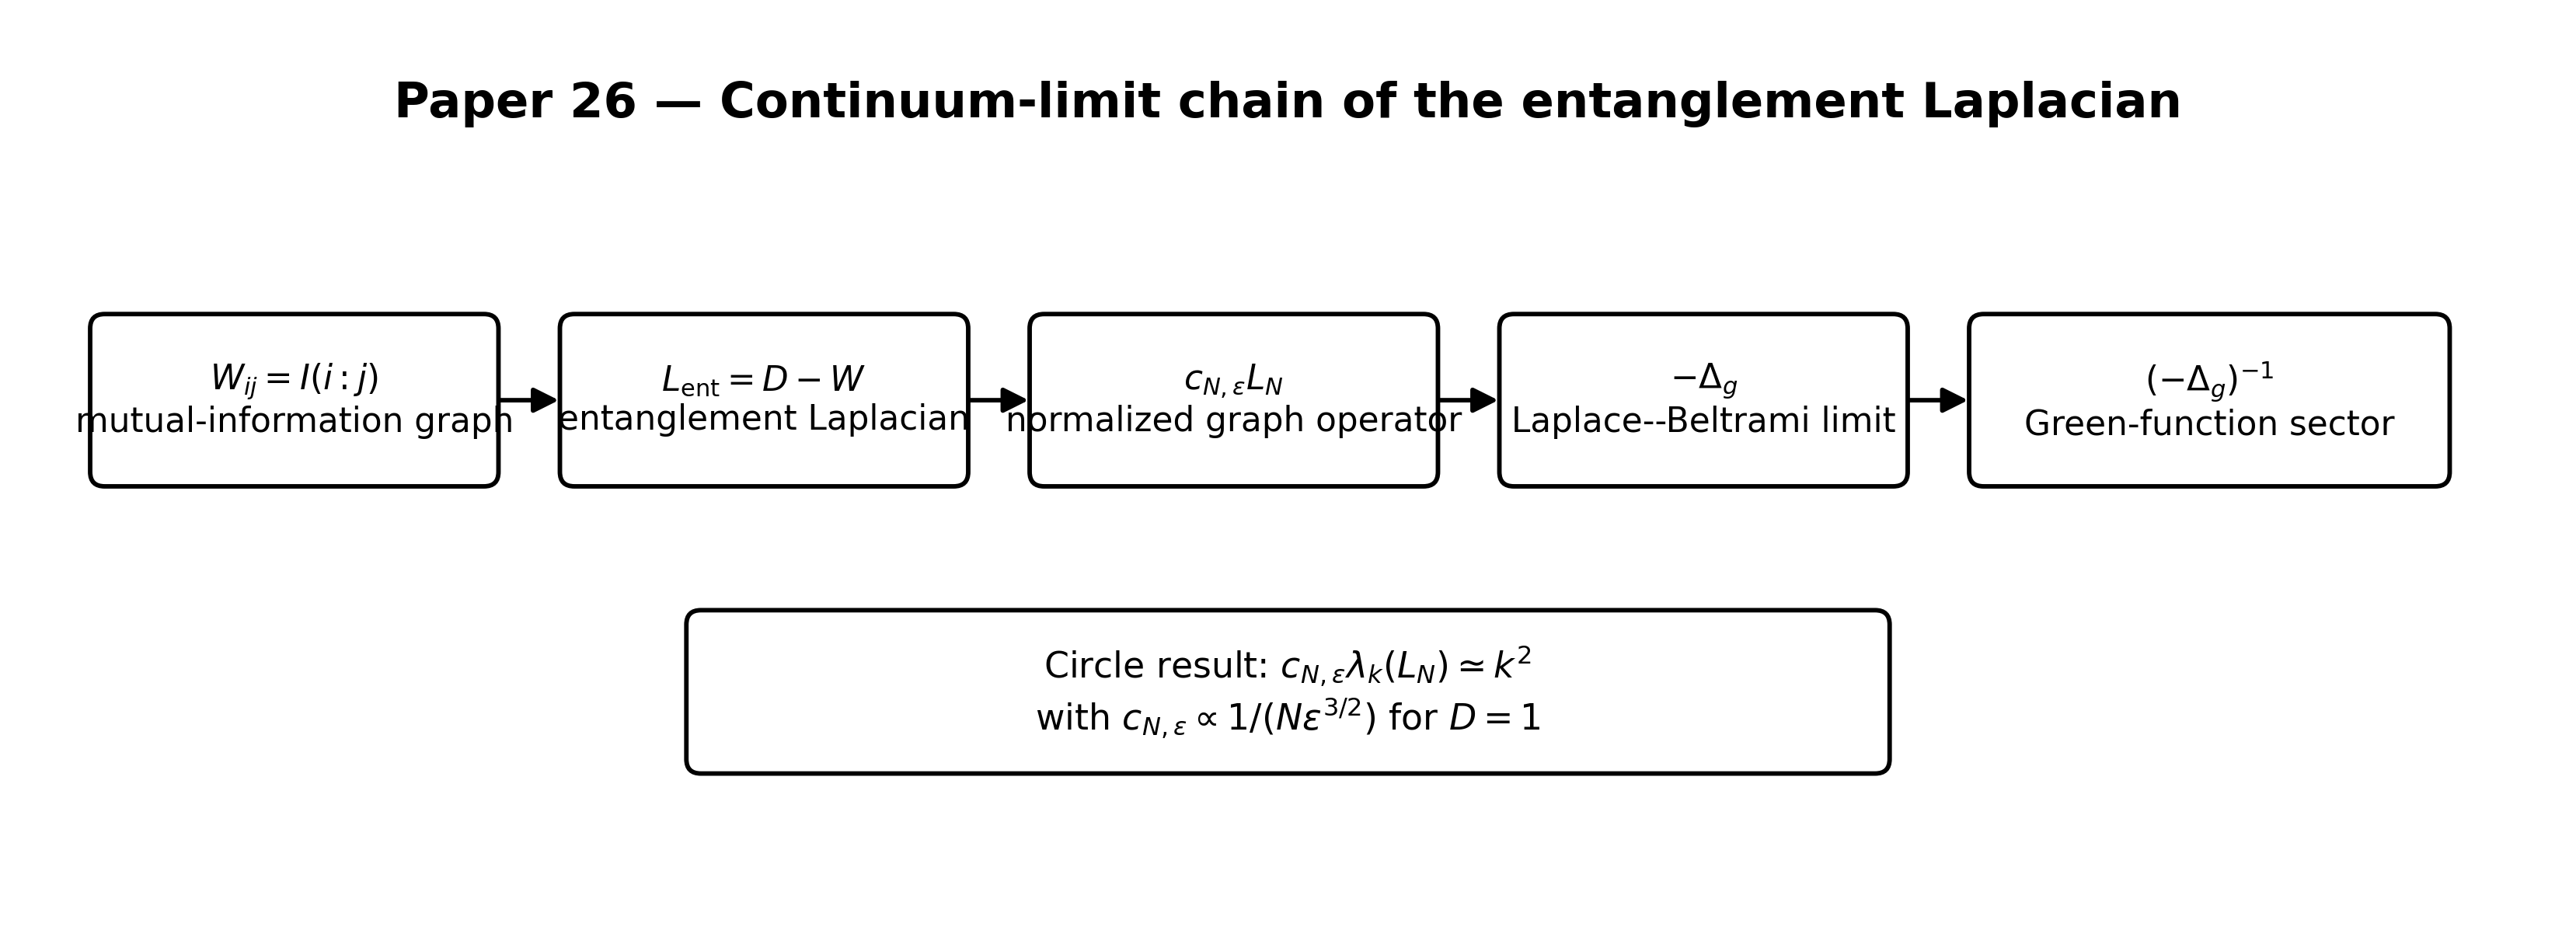
\includegraphics[width=\textwidth]{figures/fig01_limit_chain.png}
\caption{
Continuum-limit chain tested in Paper 26. The goal is to normalize the
entanglement graph Laplacian so that it converges to the Laplace--Beltrami
operator, thereby supporting the Green-function sector used in the weak-field
BuP programme.
}
\label{fig:limit-chain}
\end{figure}

\section{Role in the BuP programme}

The convergence of the entanglement Laplacian controls the chain
\begin{equation}
W_{ij}
\longrightarrow
L_{\rm ent}
\longrightarrow
-\Delta_g
\longrightarrow
(-\Delta_g)^{-1}
\longrightarrow
\Phi_{\rm BuP}.
\end{equation}

This chain supports several later components of the programme:

\begin{itemize}
\item the weak-field Green-function construction;
\item the effective propagator law;
\item the galactic and lensing sectors;
\item the correction tensor \(\mathcal H_{\mu\nu}^{\rm BuP}\);
\item the effective Einstein-limit target of Paper 25.
\end{itemize}

Thus Paper 26 addresses a narrow but crucial question:

\begin{quote}
\emph{Under what normalization does a local entanglement graph Laplacian become
the Laplace--Beltrami operator?}
\end{quote}

\section{Kernel graph setup}

Let \(M\) be a compact \(D\)-dimensional Riemannian manifold with metric \(g\).
Let \(x_i\in M\), \(i=1,\dots,N\), be sampled with node density \(\rho\). We first
consider the locally uniform case
\begin{equation}
\rho=\frac{N}{\Vol(M)}.
\end{equation}

Define the local Gaussian kernel
\begin{equation}
W_{ij}^{(\epsilon)}
=
\exp\left[
-\frac{d_g(x_i,x_j)^2}{4\epsilon}
\right],
\end{equation}
with the diagonal removed,
\begin{equation}
W_{ii}=0.
\end{equation}

The unnormalized graph Laplacian is
\begin{equation}
(L_{N,\epsilon}f)_i
=
\sum_j W_{ij}^{(\epsilon)}(f_i-f_j).
\end{equation}

This sign convention makes \(L_{N,\epsilon}\) positive semidefinite and its
continuum limit the positive operator \(-\Delta_g\).

\section{Continuum expansion}

In local normal coordinates around \(x\), set \(u=y-x\). For a smooth test
function \(f\),
\begin{equation}
f(x+u)
=
f(x)
+
u^a\partial_a f(x)
+
\frac12 u^a u^b\partial_a\partial_b f(x)
+
O(|u|^3).
\end{equation}

The graph Laplacian is approximated by
\begin{equation}
L_{N,\epsilon}f(x)
\simeq
\rho
\int_{\mathbb R^D}
e^{-|u|^2/(4\epsilon)}
\left[
f(x)-f(x+u)
\right]\dd^D u.
\end{equation}

The first-order term vanishes by symmetry,
\begin{equation}
\int_{\mathbb R^D}u^a e^{-|u|^2/(4\epsilon)}\dd^D u=0.
\end{equation}

The second-order Gaussian moment is
\begin{equation}
\int_{\mathbb R^D}
u^a u^b e^{-|u|^2/(4\epsilon)}\dd^D u
=
2\epsilon(4\pi\epsilon)^{D/2}\delta^{ab}.
\end{equation}

Therefore
\begin{align}
L_{N,\epsilon}f(x)
&\simeq
-\rho
\frac12
\partial_a\partial_b f(x)
\int_{\mathbb R^D}
u^a u^b e^{-|u|^2/(4\epsilon)}\dd^D u,
\\
&=
-\rho
\epsilon(4\pi\epsilon)^{D/2}
\Delta_g f(x).
\end{align}

Thus
\begin{equation}
\boxed{
L_{N,\epsilon}f
\simeq
-\rho(4\pi)^{D/2}\epsilon^{D/2+1}\Delta_g f.
}
\label{eq:core-expansion}
\end{equation}

\section{General normalization law}

Equation \eqref{eq:core-expansion} implies the normalization
\begin{equation}
\boxed{
c_{N,\epsilon}
=
\frac{1}
{\rho(4\pi)^{D/2}\epsilon^{D/2+1}},
\qquad
\rho=\frac{N}{\Vol(M)}.
}
\label{eq:general-normalization}
\end{equation}

Equivalently,
\begin{equation}
c_{N,\epsilon}
=
\frac{\Vol(M)}
{N(4\pi)^{D/2}\epsilon^{D/2+1}}.
\end{equation}

With this convention,
\begin{equation}
\boxed{
c_{N,\epsilon}L_{N,\epsilon}f
\to
-\Delta_g f
}
\end{equation}
in the locally uniform density regime.

\begin{figure}[htbp]
\centering
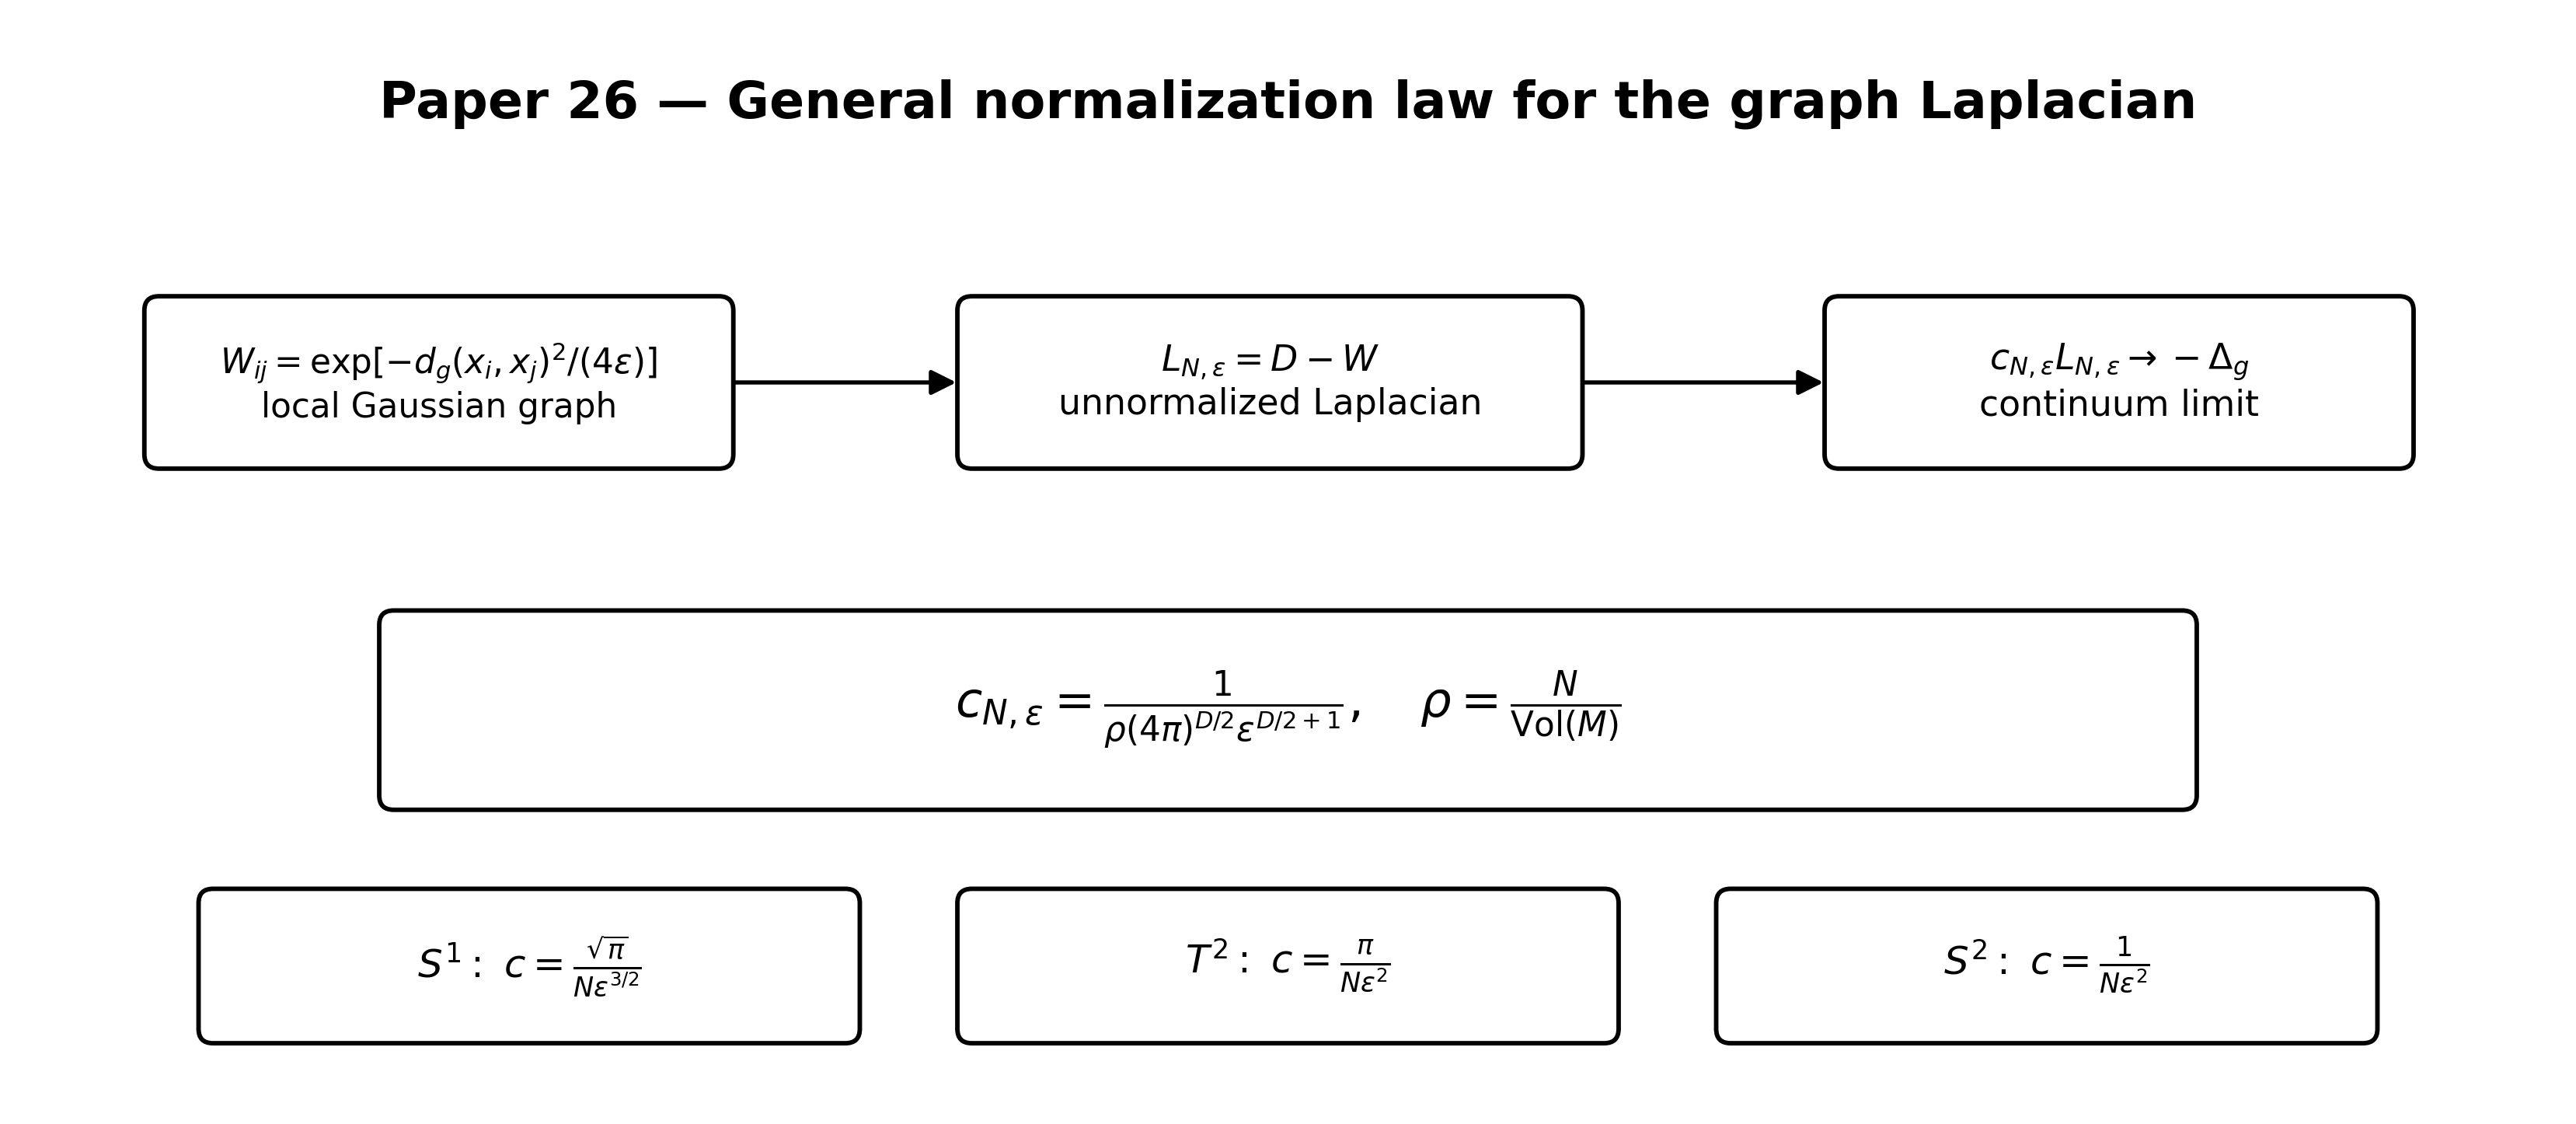
\includegraphics[width=\textwidth]{figures/fig05_general_normalization_law.png}
\caption{
General normalization law for the unnormalized local Gaussian graph Laplacian.
The normalization depends on the node density, the dimension and the kernel
scale.
}
\label{fig:general-law}
\end{figure}

\section{Validation on \(S^1\)}

For the unit circle,
\begin{equation}
\Vol(S^1)=2\pi,\qquad D=1,\qquad \rho=\frac{N}{2\pi}.
\end{equation}

The general formula gives
\begin{equation}
c_{N,\epsilon}^{S^1}
=
\frac{1}
{
\frac{N}{2\pi}(4\pi)^{1/2}\epsilon^{3/2}
}
=
\boxed{
\frac{\sqrt{\pi}}{N\epsilon^{3/2}}.
}
\end{equation}

The continuum spectrum of \(-\dd^2/\dd\theta^2\) is
\begin{equation}
0,\quad 1,1,\quad 4,4,\quad 9,9,\ldots.
\end{equation}

The numerical experiment estimates the normalization from the first nonzero
spectral band and compares the normalized low spectrum with \(k^2\).

The best prefactor result is
\begin{equation}
c_{N,\epsilon}N\epsilon^{3/2}=1.7746703414,
\end{equation}
to be compared with
\begin{equation}
\sqrt{\pi}=1.7724538509.
\end{equation}

The relative prefactor error is
\begin{equation}
1.25\times10^{-3}.
\end{equation}

The low-spectrum relative errors are
\begin{equation}
\text{mean}=1.23\%,
\qquad
\text{max}=2.94\%.
\end{equation}

\begin{figure}[htbp]
\centering
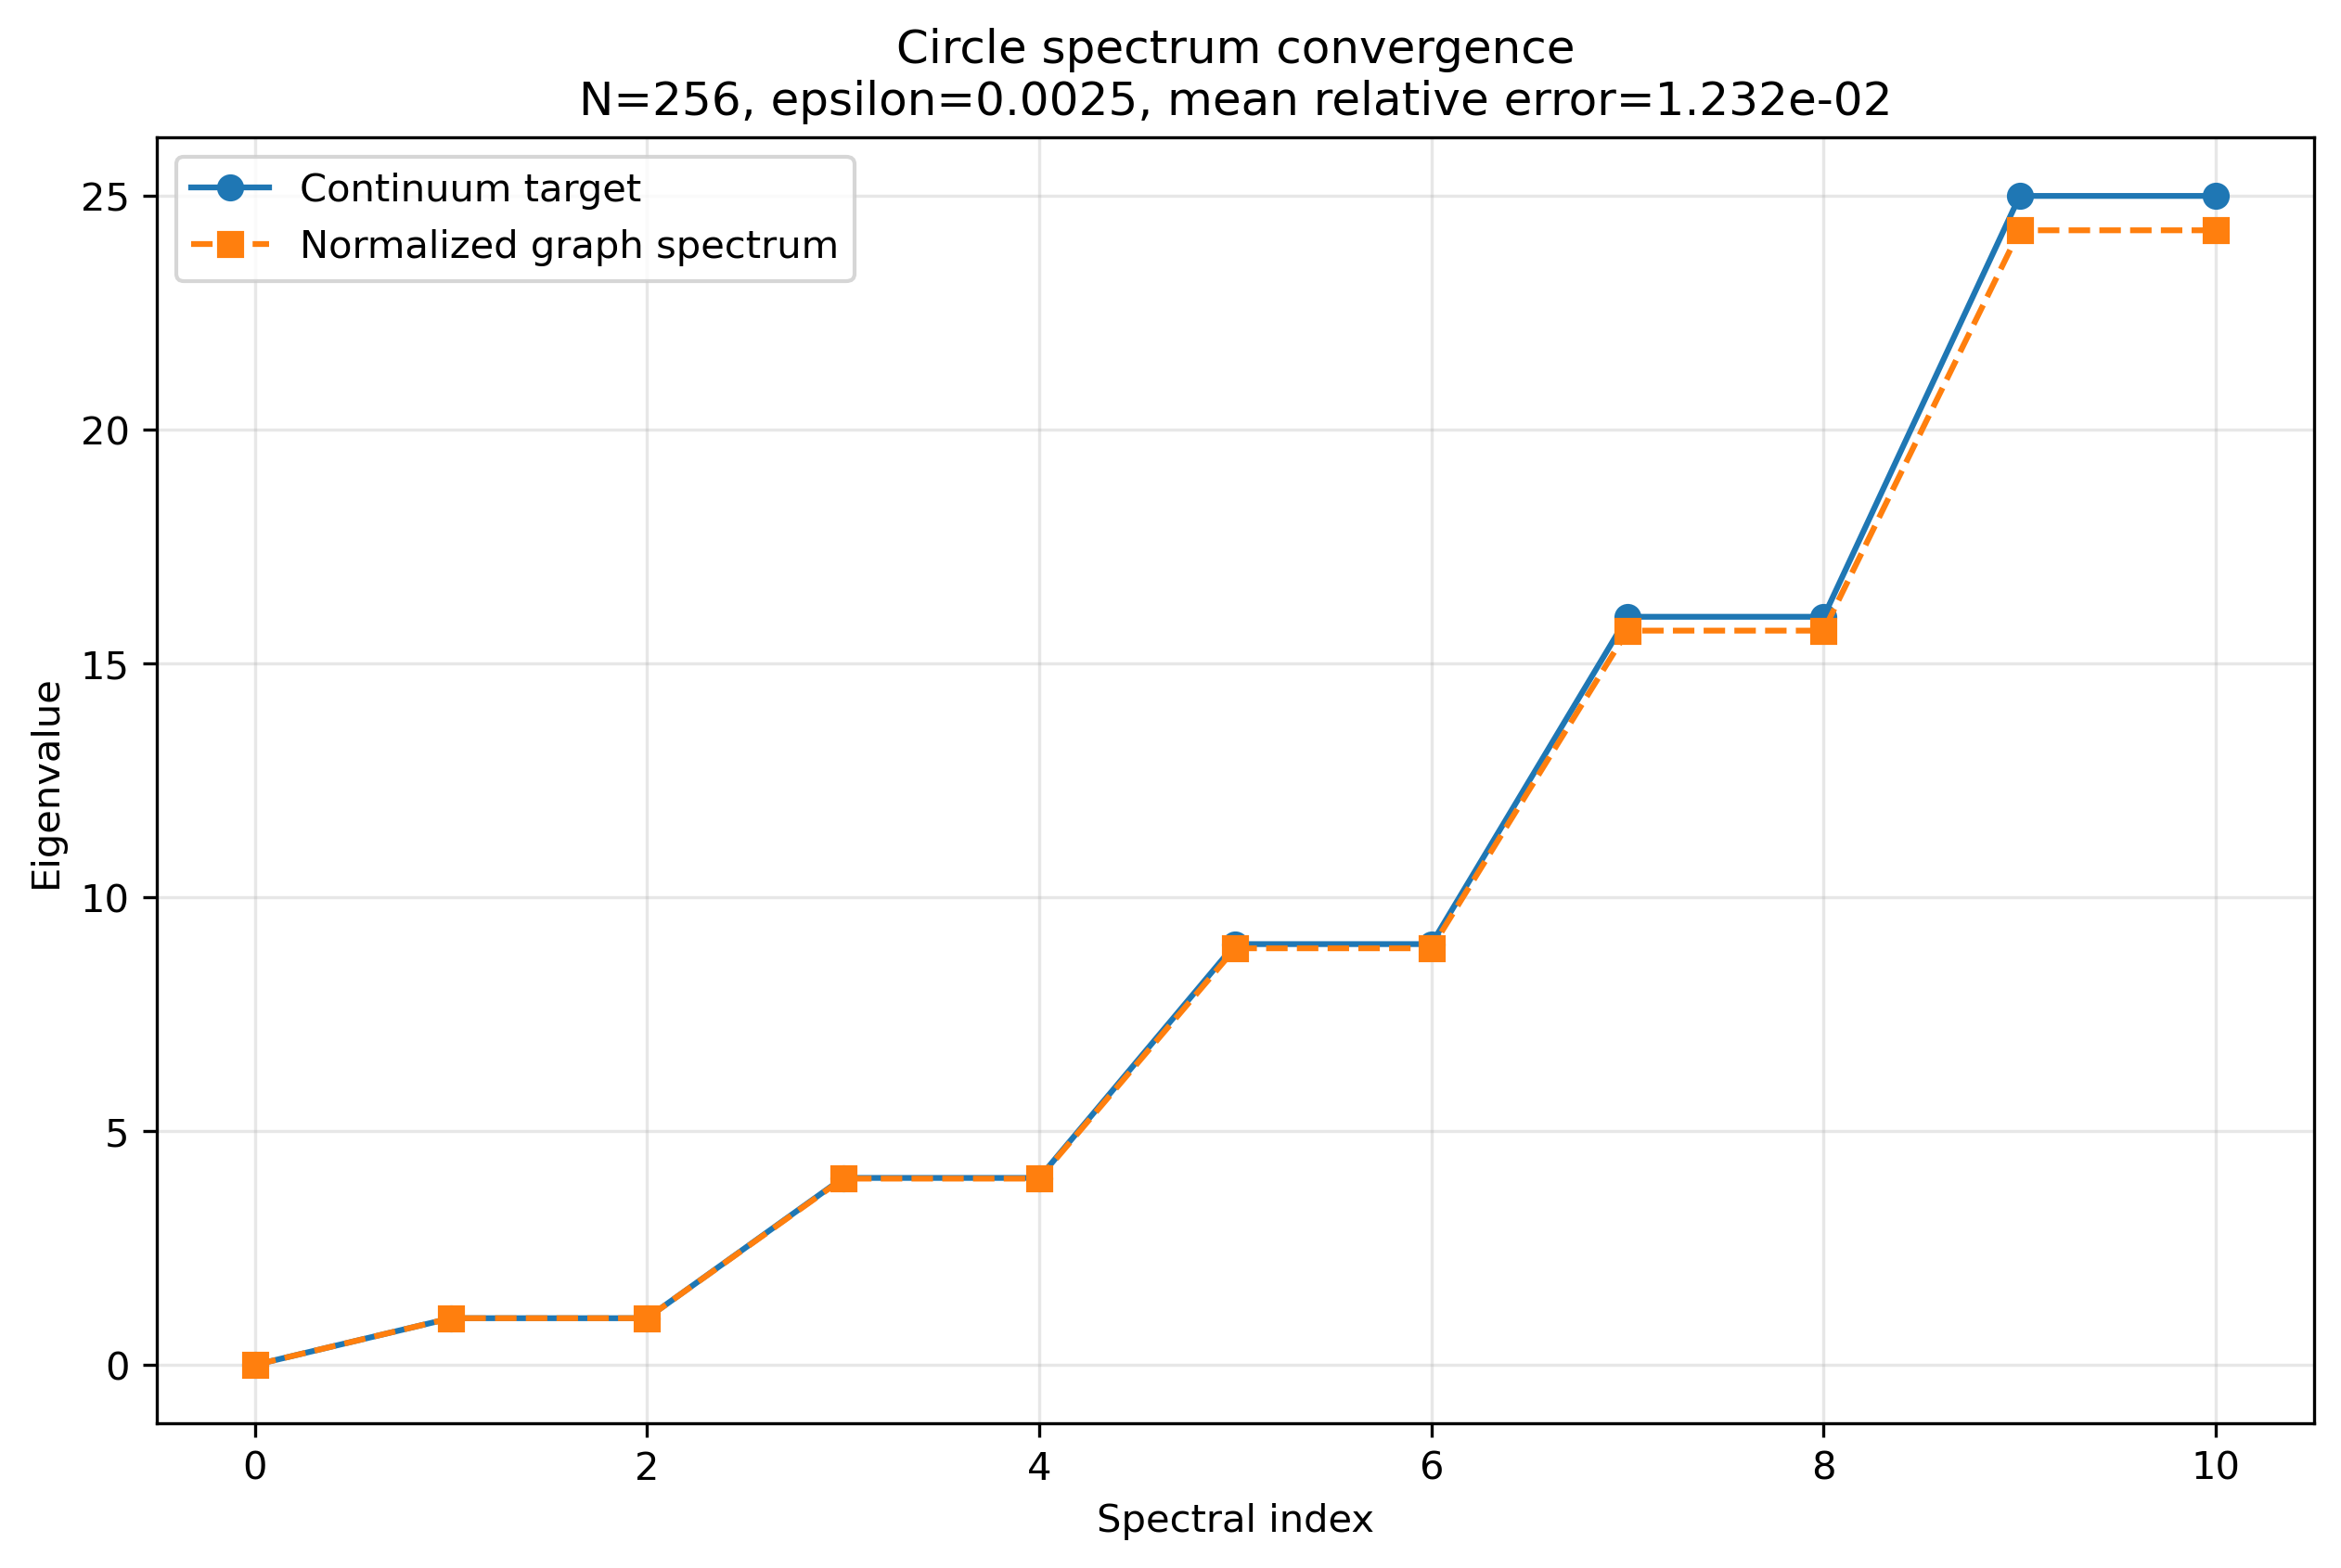
\includegraphics[width=0.86\textwidth]{figures/fig02_circle_spectrum_convergence.png}
\caption{
Low-spectrum convergence on the unit circle. After normalization by
\(\sqrt{\pi}/(N\epsilon^{3/2})\), the graph spectrum agrees with the target
spectrum \(k^2\) at the percent level.
}
\label{fig:s1-spectrum}
\end{figure}

\section{Validation on \(T^2\)}

For the flat square torus \(T^2=[0,2\pi)^2\),
\begin{equation}
\Vol(T^2)=4\pi^2,\qquad D=2,\qquad \rho=\frac{N}{4\pi^2}.
\end{equation}

The normalization is therefore
\begin{equation}
c_{N,\epsilon}^{T^2}
=
\frac{1}
{
\frac{N}{4\pi^2}(4\pi)\epsilon^2
}
=
\boxed{
\frac{\pi}{N\epsilon^2}.
}
\end{equation}

The continuum spectrum of the positive Laplacian on \(T^2\) is
\begin{equation}
\lambda_{m,n}=m^2+n^2.
\end{equation}

Because a regular periodic grid is block-circulant, the spectrum can be
computed efficiently by FFT. The corrected \(T^2\) experiment gives
\begin{equation}
c_{N,\epsilon}N\epsilon^2=3.1573267968,
\end{equation}
to be compared with
\begin{equation}
\pi=3.1415926536.
\end{equation}

The relative prefactor error is
\begin{equation}
0.5008\%.
\end{equation}

The low-spectrum relative errors with the theoretical normalization are
\begin{equation}
\text{mean}=2.46\%,
\qquad
\text{max}=4.84\%.
\end{equation}

\section{Validation on \(S^2\)}

For the unit sphere,
\begin{equation}
\Vol(S^2)=4\pi,\qquad D=2,\qquad \rho=\frac{N}{4\pi}.
\end{equation}

The general law gives
\begin{equation}
c_{N,\epsilon}^{S^2}
=
\frac{1}
{
\frac{N}{4\pi}(4\pi)\epsilon^2
}
=
\boxed{
\frac{1}{N\epsilon^2}.
}
\end{equation}

The continuum spectrum is
\begin{equation}
\lambda_\ell=\ell(\ell+1),
\qquad
\text{multiplicity }2\ell+1.
\end{equation}

The tested low spectrum is therefore
\begin{equation}
0,\quad 2,2,2,\quad 6,6,6,6,6,\quad 12,\ldots.
\end{equation}

Using a Fibonacci quasi-uniform sampling of the unit sphere, the best row gives
\begin{equation}
N=1024,\qquad \epsilon=0.01,
\end{equation}
with empirical prefactor
\begin{equation}
c_{N,\epsilon}N\epsilon^2=1.0201663725.
\end{equation}

The prefactor error is
\begin{equation}
2.02\%.
\end{equation}

The low-spectrum relative errors are
\begin{equation}
\text{mean}=6.85\%,
\qquad
\text{max}=10.35\%.
\end{equation}

These errors are larger than in the \(S^1\) and \(T^2\) tests because the
Fibonacci sphere is quasi-uniform but not an exact spectral grid, the graph is
not circulant, and the spherical eigenvalues have nontrivial multiplicities.

\begin{figure}[htbp]
\centering
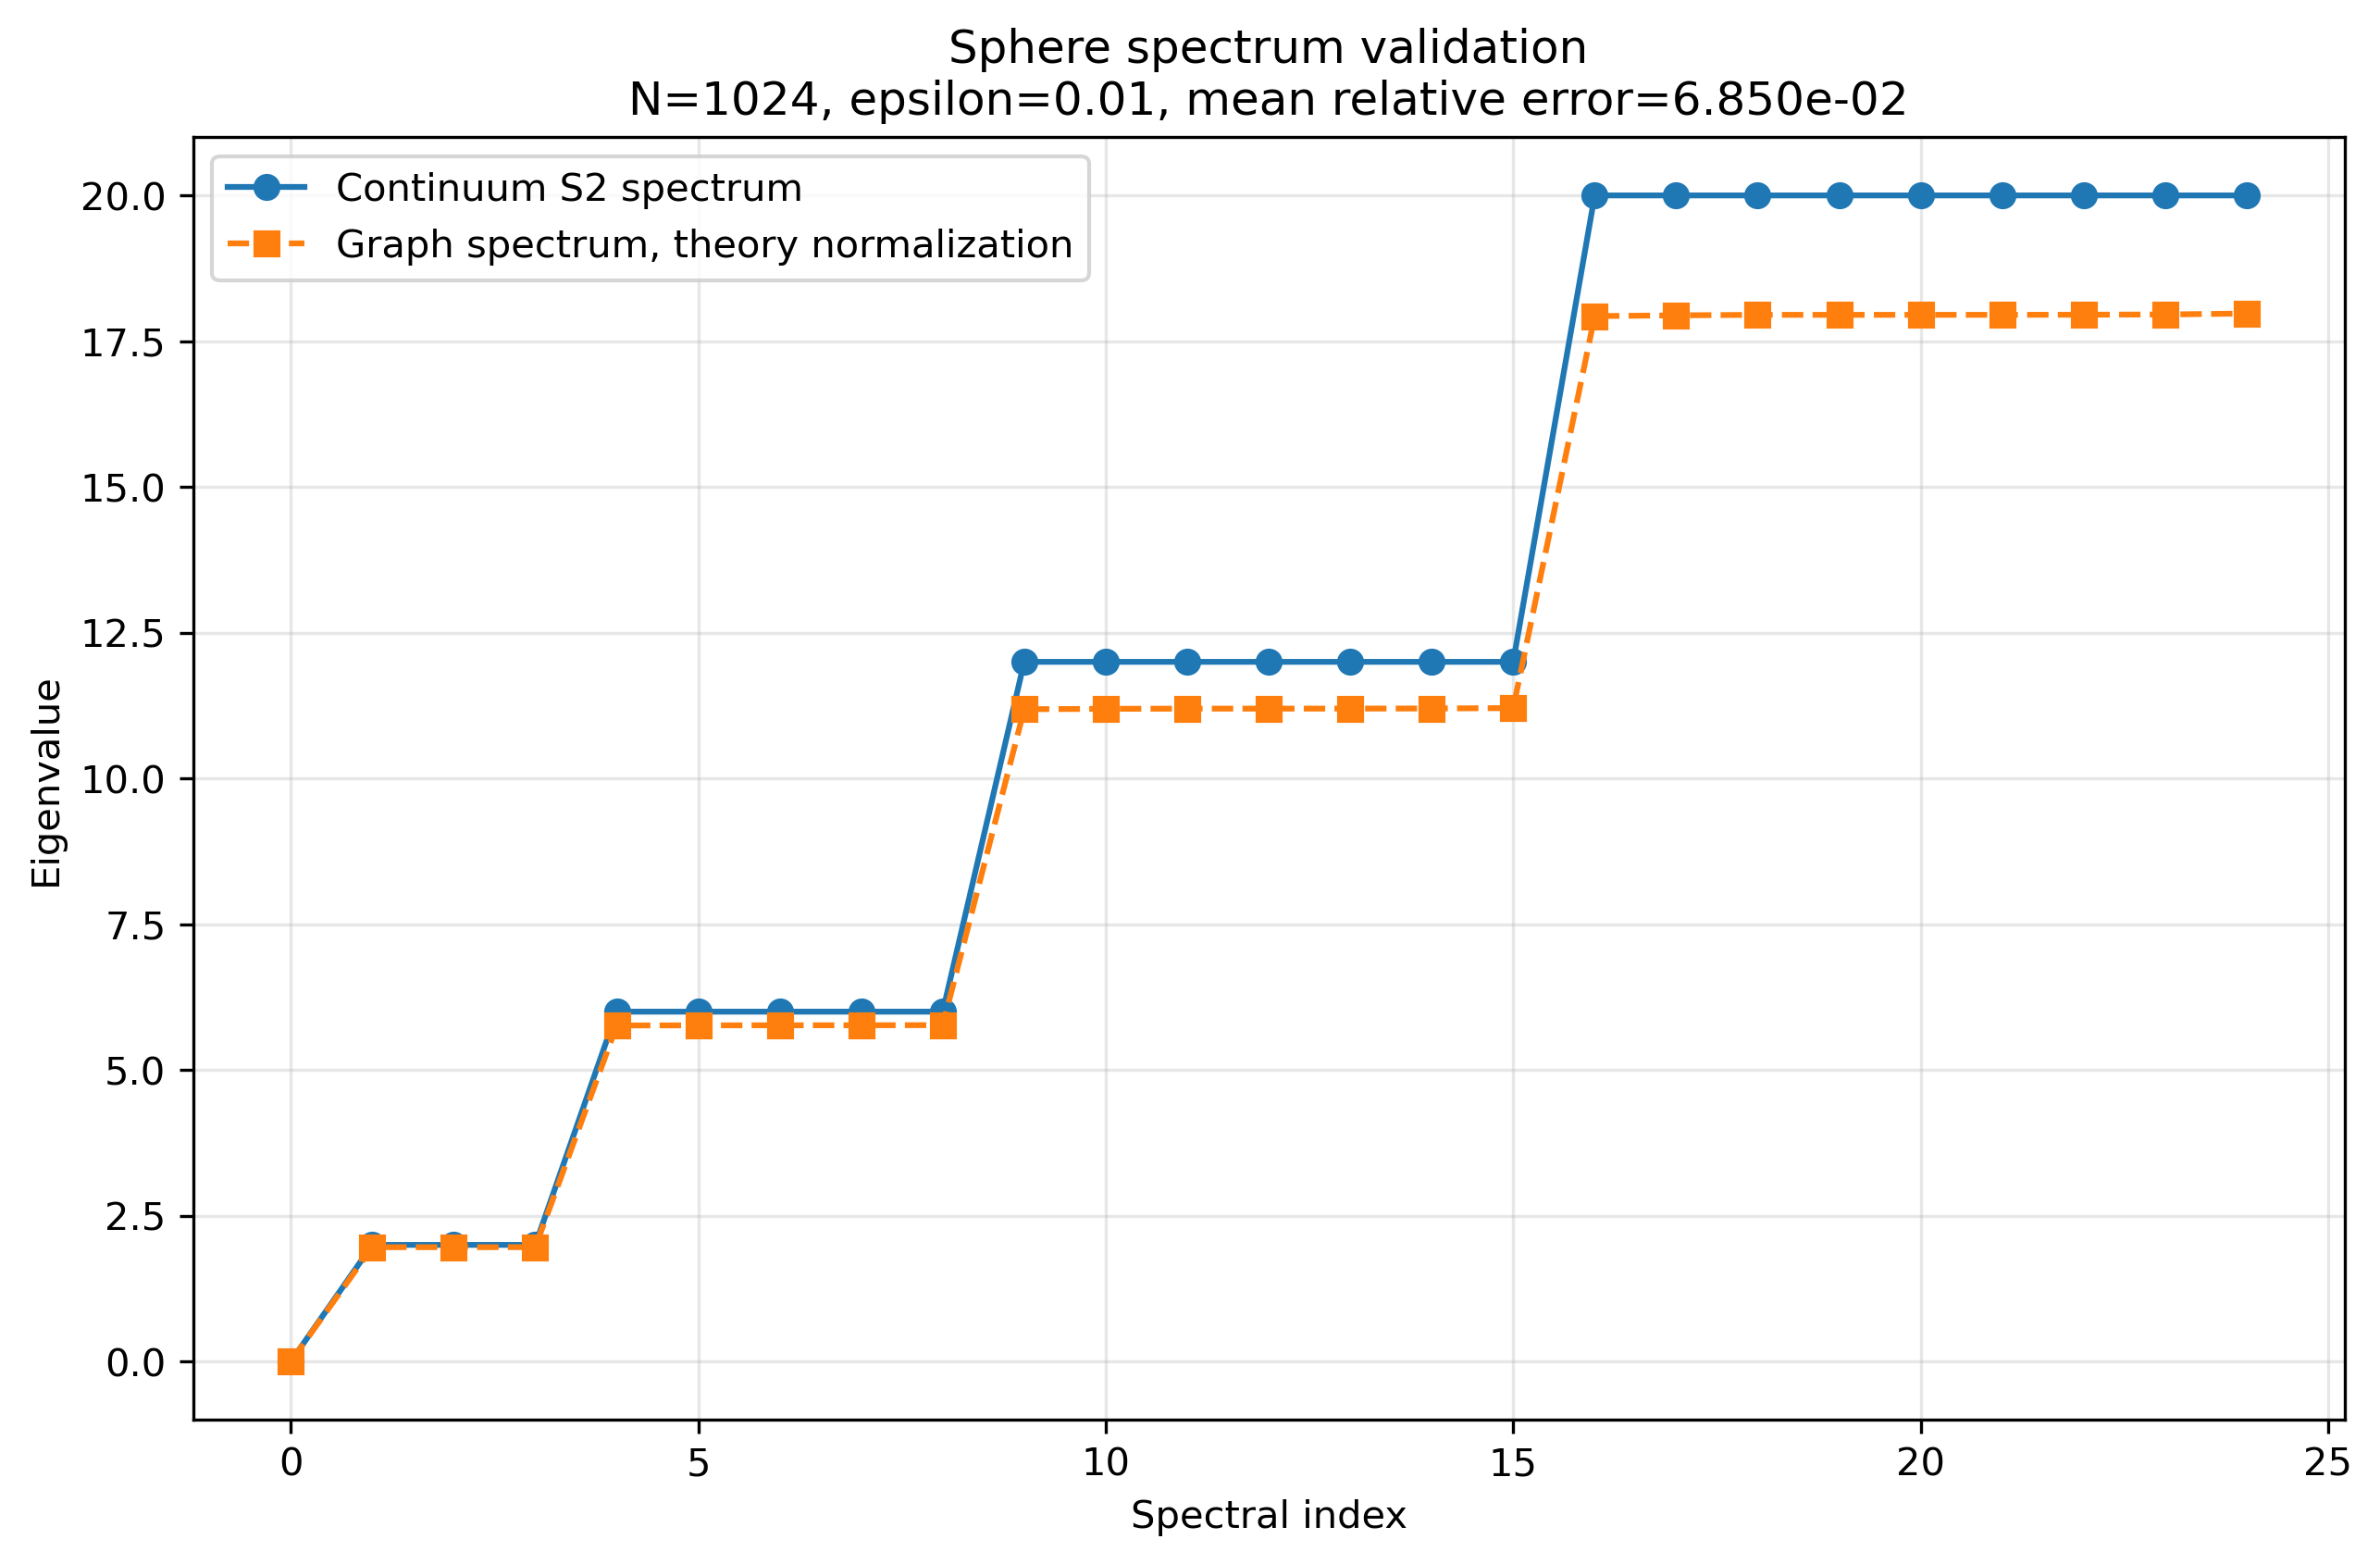
\includegraphics[width=0.86\textwidth]{figures/fig07_sphere_spectrum_validation.png}
\caption{
Low-spectrum validation on the unit sphere. The result confirms the predicted
normalization \(1/(N\epsilon^2)\), with larger finite-\(N\) and sampling errors
than in the flat periodic cases.
}
\label{fig:s2-spectrum}
\end{figure}

\section{Summary of the three uniform tests}

The three controlled tests validate the same general normalization law:
\begin{equation}
c_{N,\epsilon}
=
\frac{1}
{\rho(4\pi)^{D/2}\epsilon^{D/2+1}}.
\end{equation}

\begin{table}[htbp]
\centering
\begin{tabular}{llll}
\toprule
Geometry & Density \(\rho\) & Predicted \(c_{N,\epsilon}\) & Status \\
\midrule
\(S^1\) & \(N/(2\pi)\) &
\(\sqrt{\pi}/(N\epsilon^{3/2})\) &
\(0.125\%\) prefactor error \\

\(T^2\) & \(N/(4\pi^2)\) &
\(\pi/(N\epsilon^2)\) &
\(0.501\%\) prefactor error \\

\(S^2\) & \(N/(4\pi)\) &
\(1/(N\epsilon^2)\) &
\(2.02\%\) prefactor error \\
\bottomrule
\end{tabular}
\caption{
Uniform-density validation of the general normalization law. The sphere is less
sharp because of quasi-uniform sampling and curvature corrections, but still
confirms the predicted prefactor.
}
\label{tab:uniform-tests}
\end{table}

\begin{figure}[htbp]
\centering
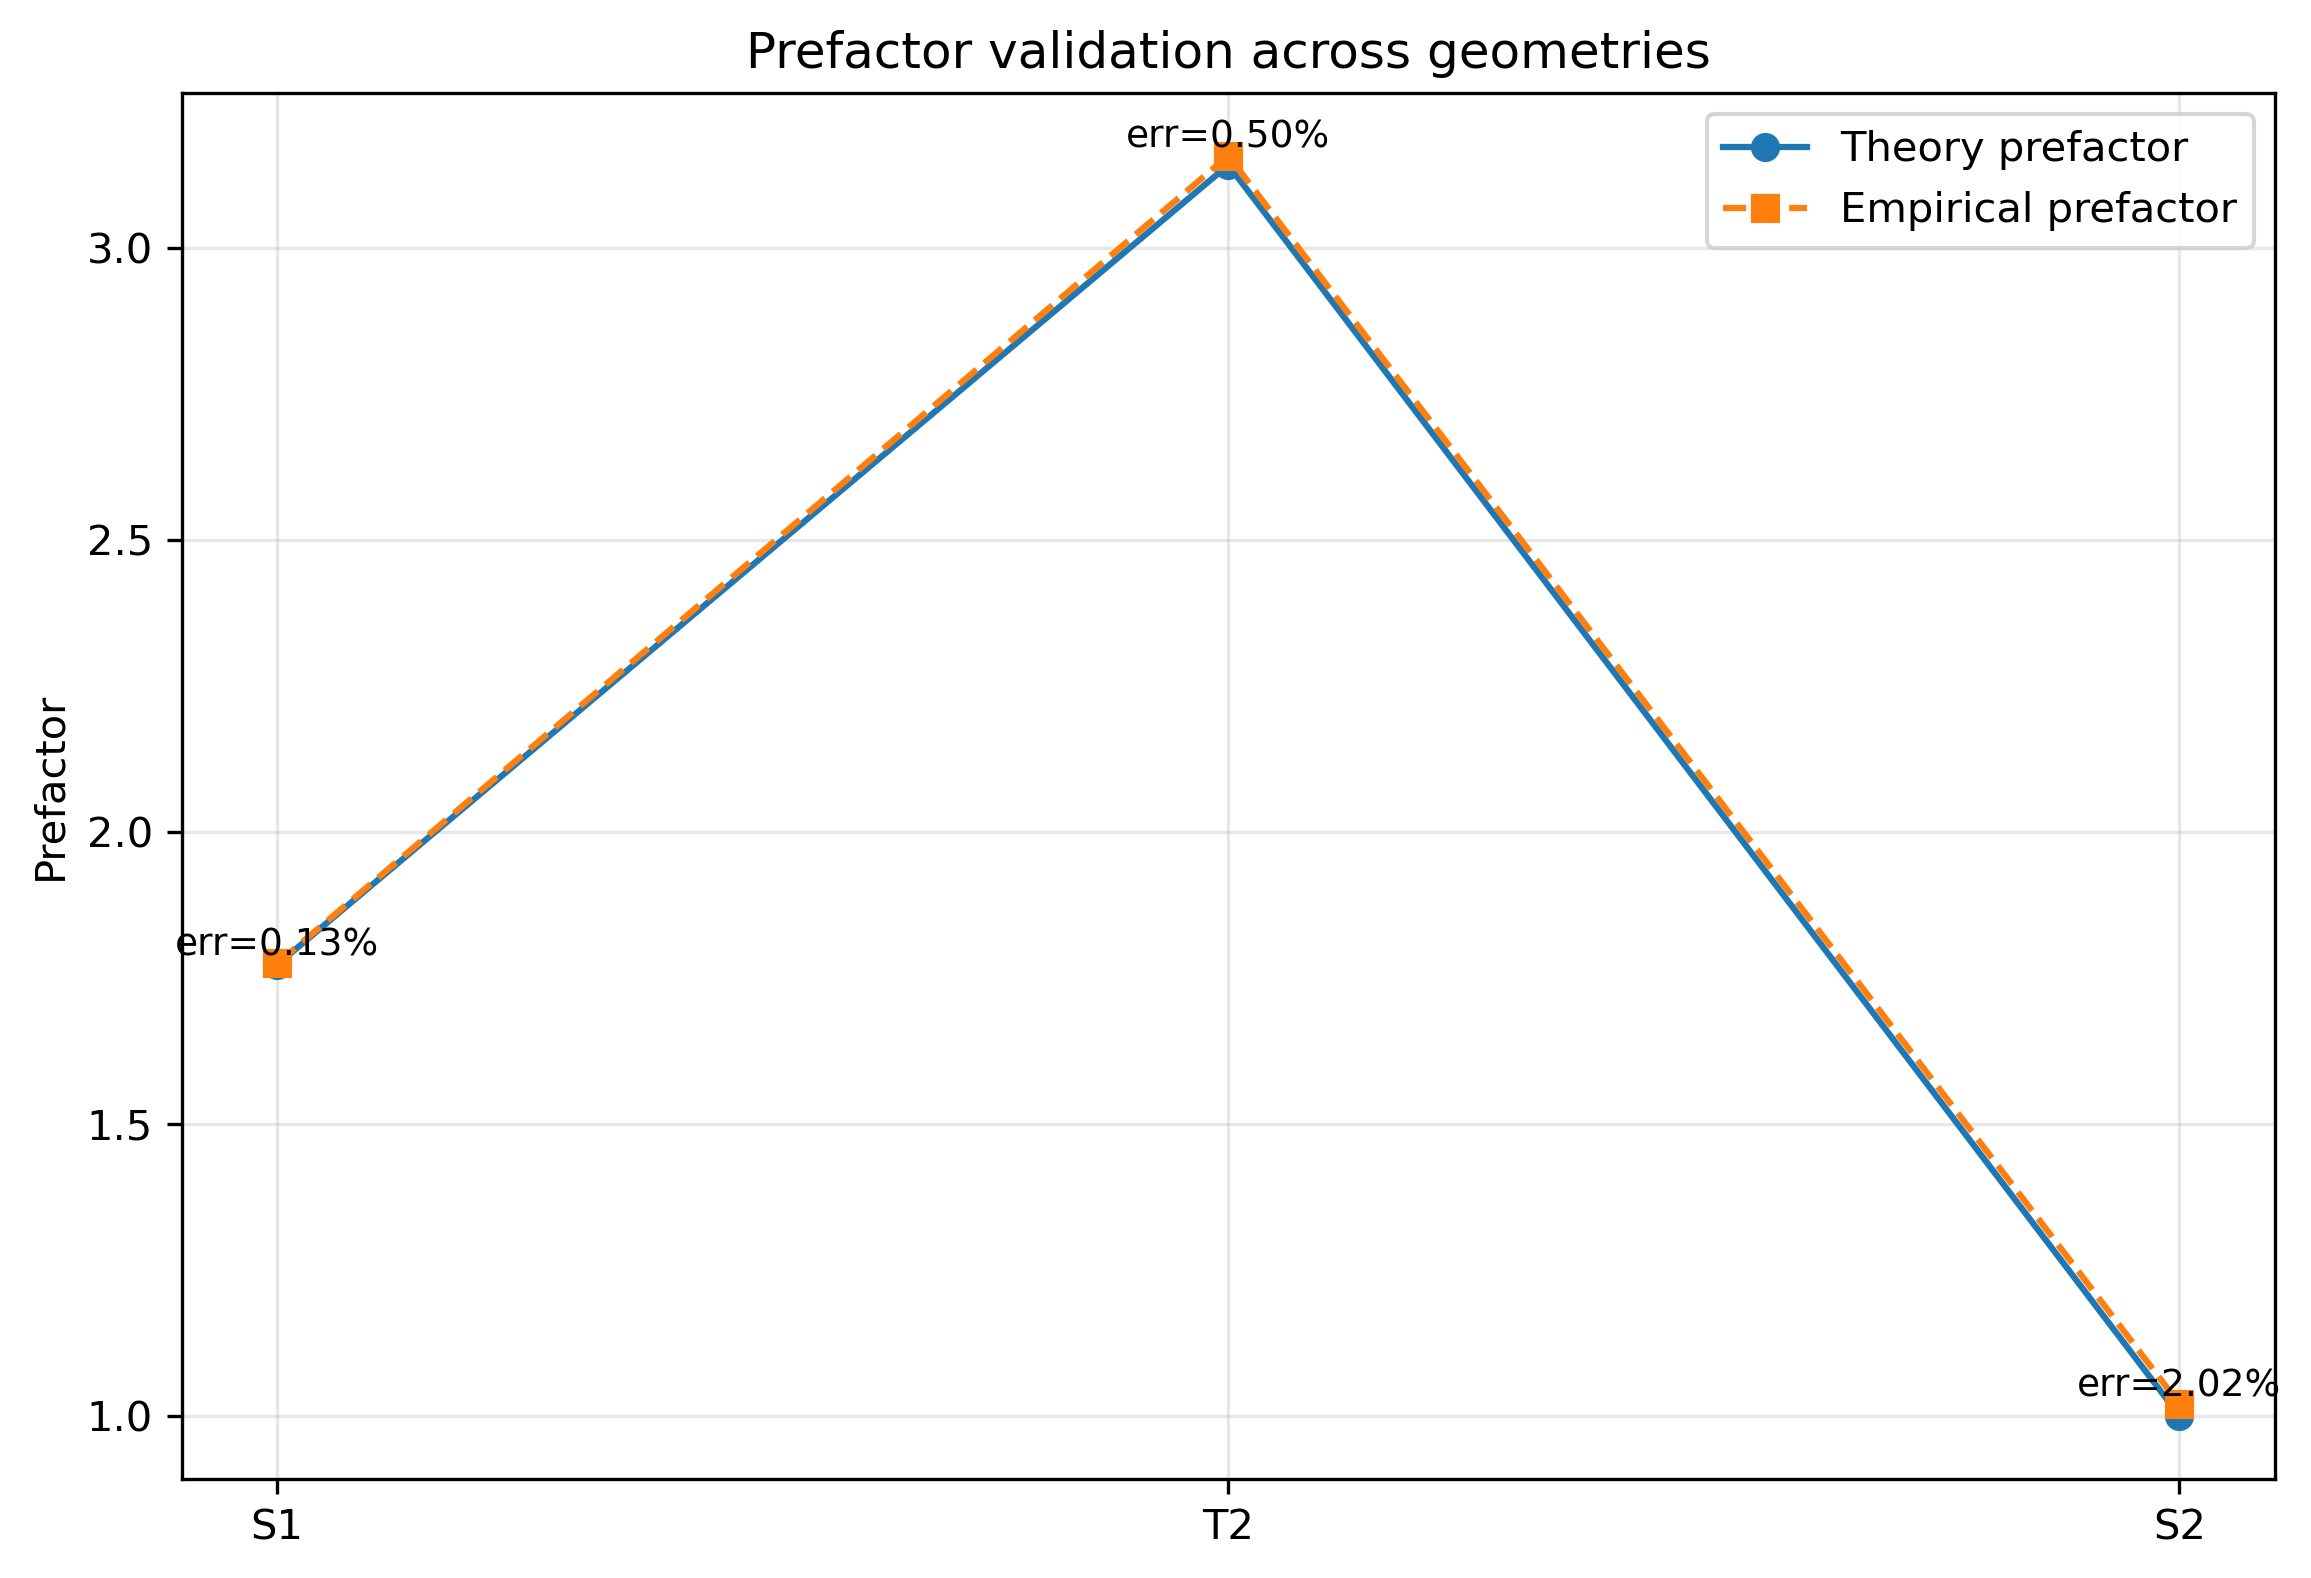
\includegraphics[width=0.82\textwidth]{figures/fig06_prefactor_validation_summary.png}
\caption{
Prefactor validation across \(S^1\), \(T^2\), and \(S^2\). The empirical
prefactors agree with the theoretical values derived from the general density
normalization law.
}
\label{fig:prefactor-summary}
\end{figure}

\section{Non-uniform density and drift bias}

The preceding result assumes locally uniform density. This assumption is
essential.

Let the density be position-dependent:
\begin{equation}
\rho=\rho(x).
\end{equation}

Then
\begin{equation}
L_{N,\epsilon}f(x)
\simeq
\rho(x)
\int
k_\epsilon(x,y)
\left[
f(x)-f(y)
\right]\dd y.
\end{equation}

Expanding both \(f\) and \(\rho\), the raw combinatorial Laplacian contains a
density drift. At leading order one obtains
\begin{equation}
L_{N,\epsilon}f
\simeq
-\rho(x)(4\pi)^{D/2}\epsilon^{D/2+1}
\left[
\Delta_g f
+
2\nabla\log\rho\cdot\nabla f
\right].
\end{equation}

After local normalization,
\begin{equation}
\boxed{
c_{N,\epsilon}(x)L_{N,\epsilon}f
\simeq
-\Delta_g f
-
2\nabla\log\rho\cdot\nabla f.
}
\label{eq:density-drift}
\end{equation}

The exact coefficient depends on the graph normalization convention, but the
existence of a density-induced drift term is structural.

\subsection{Controlled \(S^1\) density test}

We tested the non-uniform density
\begin{equation}
\rho(\theta)
=
\frac{1}{2\pi}(1+a\cos\theta),
\qquad
a=0.5,
\end{equation}
with test function
\begin{equation}
f(\theta)=\sin(2\theta).
\end{equation}

The drift term is controlled analytically:
\begin{equation}
\partial_\theta\log\rho
=
\frac{-a\sin\theta}{1+a\cos\theta}.
\end{equation}

The raw graph operator was compared to two targets:
\begin{align}
\text{pure target} &= -f''(\theta),\\
\text{drift target} &=
-f''(\theta)
-
2(\partial_\theta\log\rho)f'(\theta).
\end{align}

The best run gives
\begin{equation}
N=2048,\qquad \epsilon=0.02,
\end{equation}
with density contrast
\begin{equation}
\rho_{\max}/\rho_{\min}\simeq3.
\end{equation}

The raw operator errors are
\begin{equation}
\mathrm{RMSE}_{\rm pure}=0.3921,
\qquad
\mathrm{RMSE}_{\rm drift}=0.1738.
\end{equation}

Thus the drift target improves the fit by a factor
\begin{equation}
2.26.
\end{equation}

\begin{figure}[htbp]
\centering
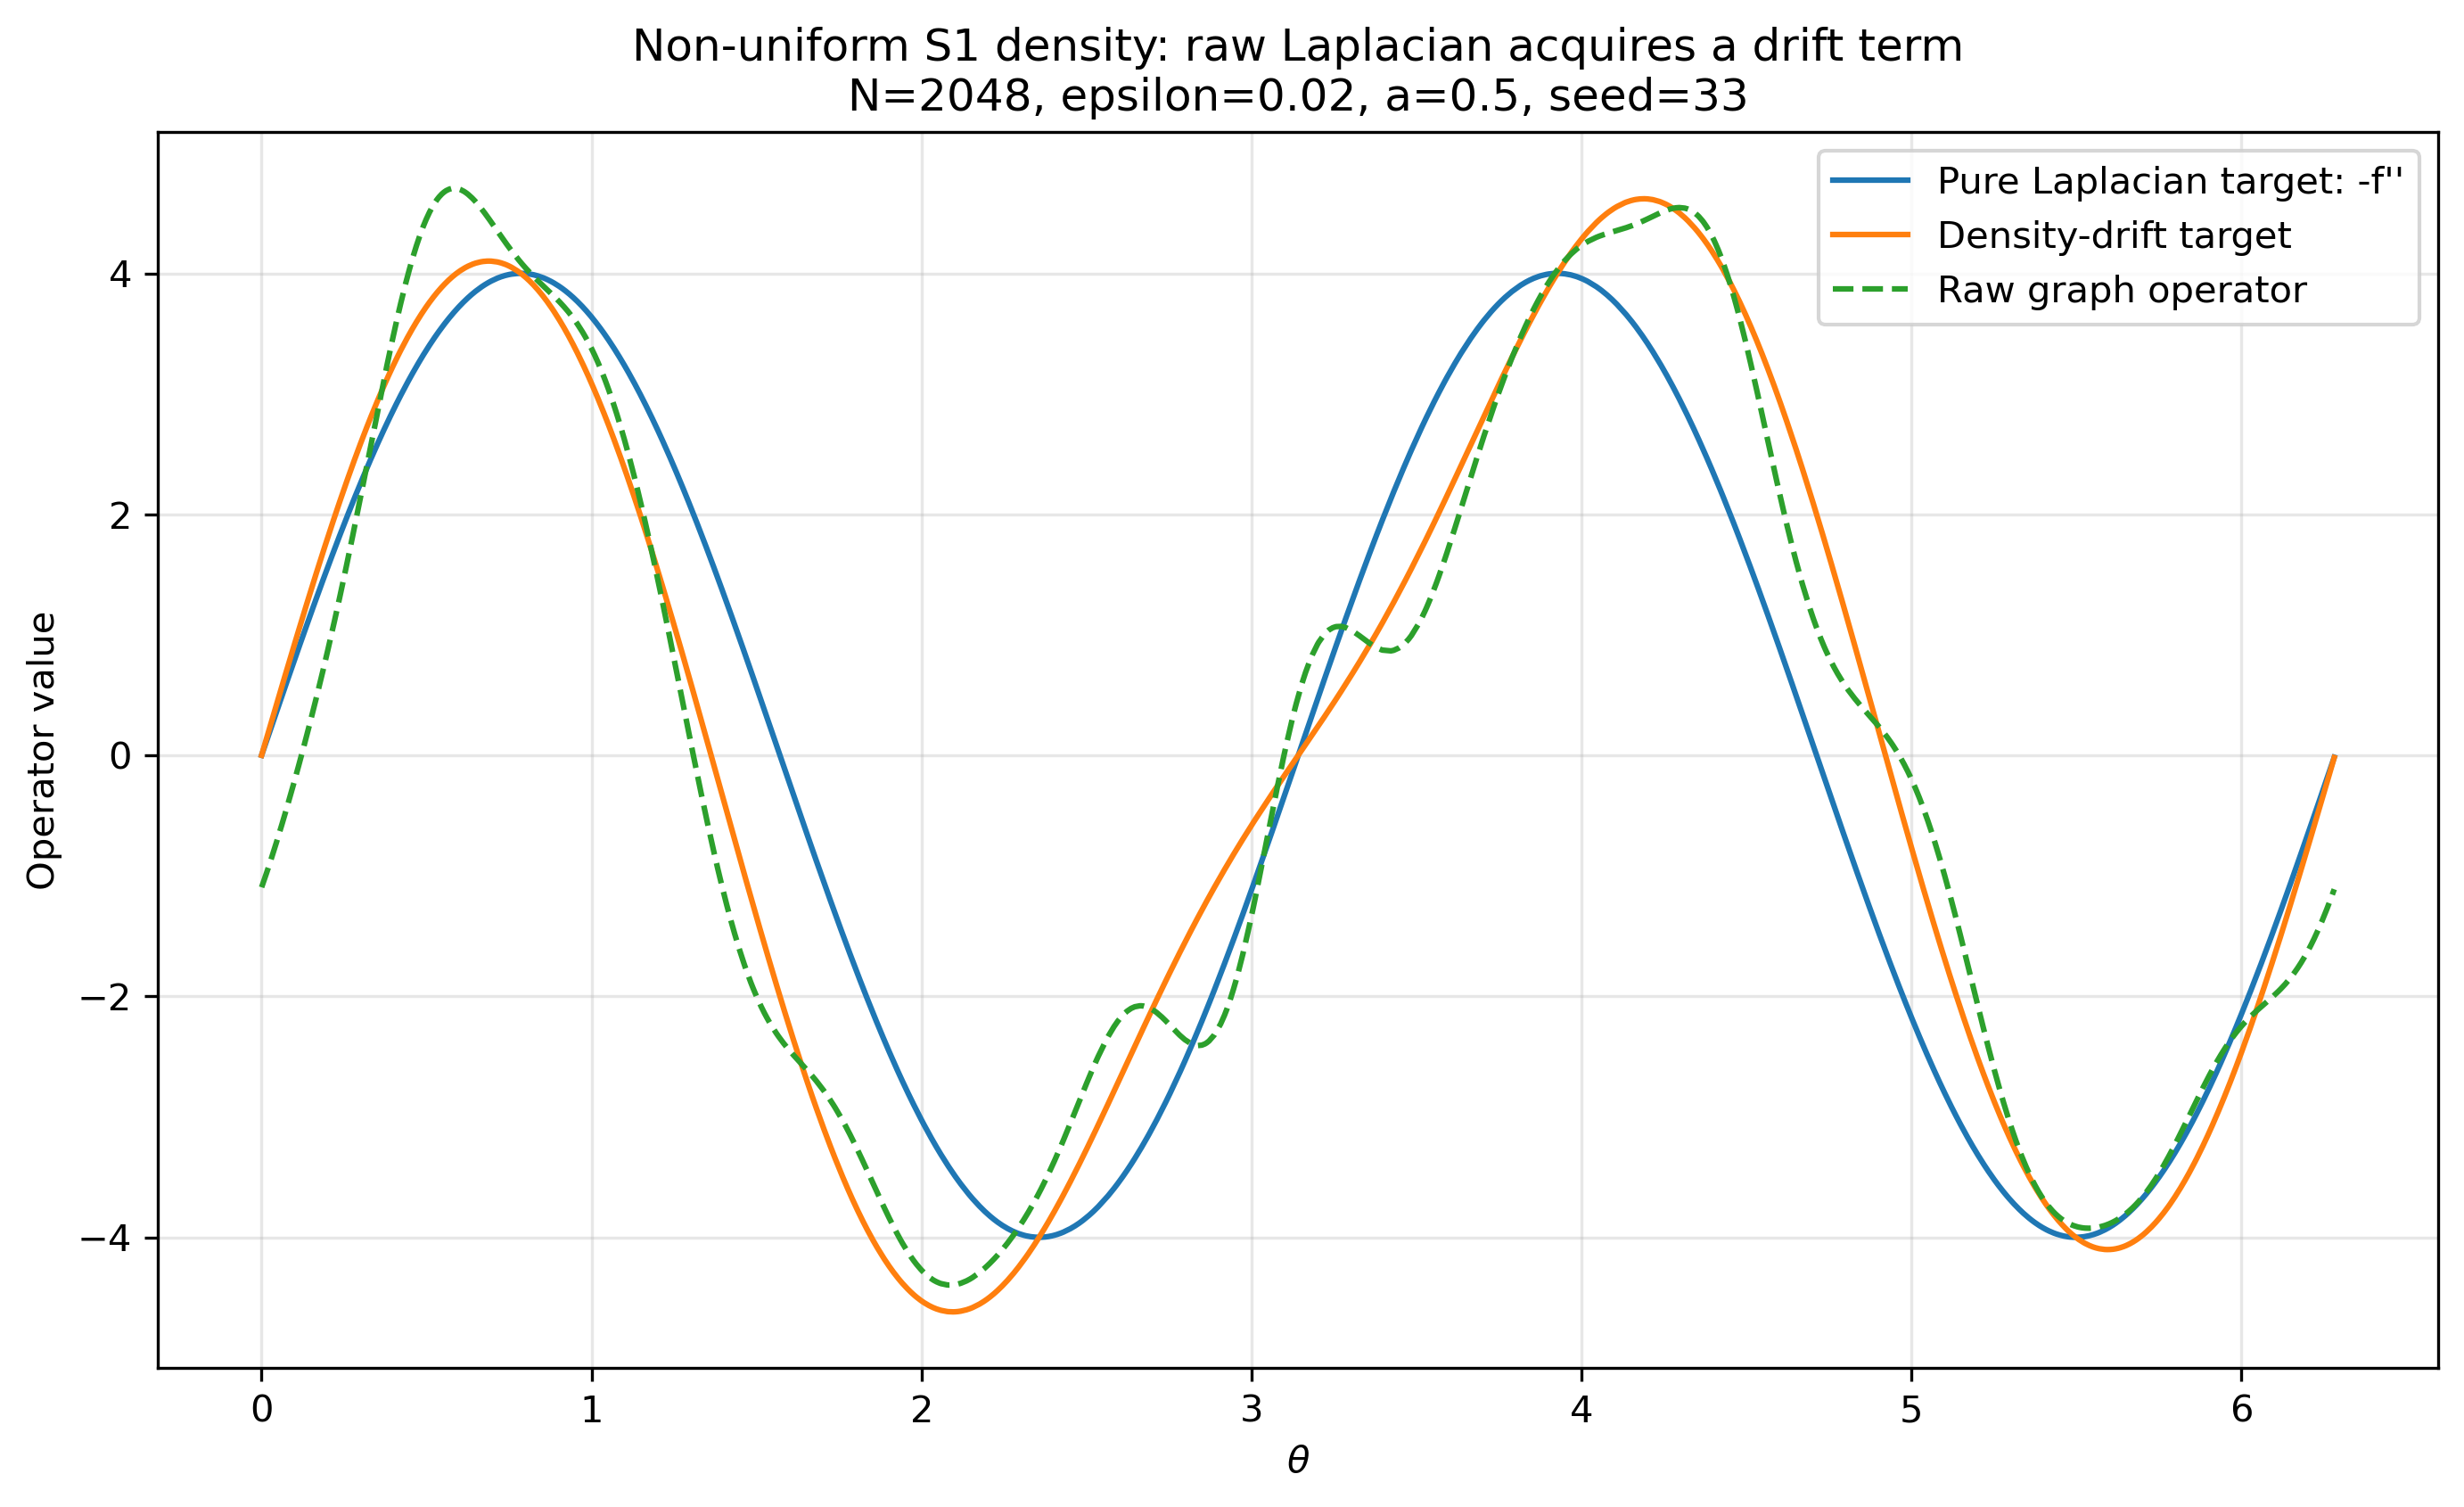
\includegraphics[width=0.92\textwidth]{figures/fig08_nonuniform_s1_density_drift.png}
\caption{
Controlled non-uniform \(S^1\) density test. The raw graph Laplacian agrees
better with the density-drift operator than with the pure Laplacian target.
}
\label{fig:nonuniform-drift}
\end{figure}

\section{Density-corrected Laplacians: two conventions}

The density-bias test shows that the raw combinatorial Laplacian should not be
used blindly in non-uniform sampling regimes. However, density correction is
convention-dependent. Two graph-operator conventions must be distinguished:

\begin{enumerate}
\item a symmetric combinatorial correction,
\[
L_{\rm comb}^{(\alpha)}
=
D^{(\alpha)}-W^{(\alpha)};
\]

\item the diffusion-maps Markov generator,
\[
G^{(\alpha)}
=
\frac{I-P^{(\alpha)}}{\epsilon}.
\]
\end{enumerate}

This distinction is essential. A finite-\(N\) correction that performs best for
the symmetric combinatorial operator is not necessarily the same correction that
is optimal for the Markov diffusion-maps generator.

\subsection{Symmetric combinatorial correction}

Define
\begin{equation}
q_i=\sum_j W_{ij}.
\end{equation}

We first tested the corrected symmetric kernel
\begin{equation}
W_{ij}^{(\alpha)}
=
\frac{W_{ij}}
{q_i^\alpha q_j^\alpha}.
\end{equation}

The associated combinatorial Laplacian is
\begin{equation}
L_{\rm comb}^{(\alpha)}
=
D^{(\alpha)}-W^{(\alpha)}.
\end{equation}

The tested cases were
\begin{equation}
\alpha=0,\qquad \alpha=\frac12,\qquad \alpha=1.
\end{equation}

The case \(\alpha=0\) is the raw graph. The case \(\alpha=1/2\) is the symmetric
degree-flattening correction
\begin{equation}
W_{ij}^{(1/2)}
=
\frac{W_{ij}}{\sqrt{q_iq_j}}.
\end{equation}

The median results are:

\begin{table}[htbp]
\centering
\begin{tabular}{rrrr}
\toprule
\(\alpha\) & Pure RMSE & Drift RMSE & Degree contrast \\
\midrule
0 & 0.4588 & 0.3803 & 3.3045 \\
0.5 & 0.2690 & 0.2916 & 1.0622 \\
1 & 0.3931 & 0.5163 & 3.0197 \\
\bottomrule
\end{tabular}
\caption{
Density-corrected non-uniform \(S^1\) test for the symmetric combinatorial
operator \(D^{(\alpha)}-W^{(\alpha)}\). In this finite-\(N\) convention,
\(\alpha=1/2\) gives the best empirical recovery of the pure Laplacian and
nearly flattens the degree distribution.
}
\label{tab:density-correction}
\end{table}

The best pure Laplacian recovery in this symmetric combinatorial family is
\begin{equation}
\alpha=\frac12,\qquad
\epsilon=0.04,\qquad
\mathrm{RMSE}_{\rm pure}=0.16098.
\end{equation}

The degree contrast is reduced to
\begin{equation}
1.0537.
\end{equation}

This result should not be interpreted as a contradiction of diffusion-maps
theory. The operator tested here is the symmetric combinatorial Laplacian
\(D^{(\alpha)}-W^{(\alpha)}\), not the row-normalized Markov generator used in
the standard Coifman--Lafon construction.

\begin{figure}[htbp]
\centering
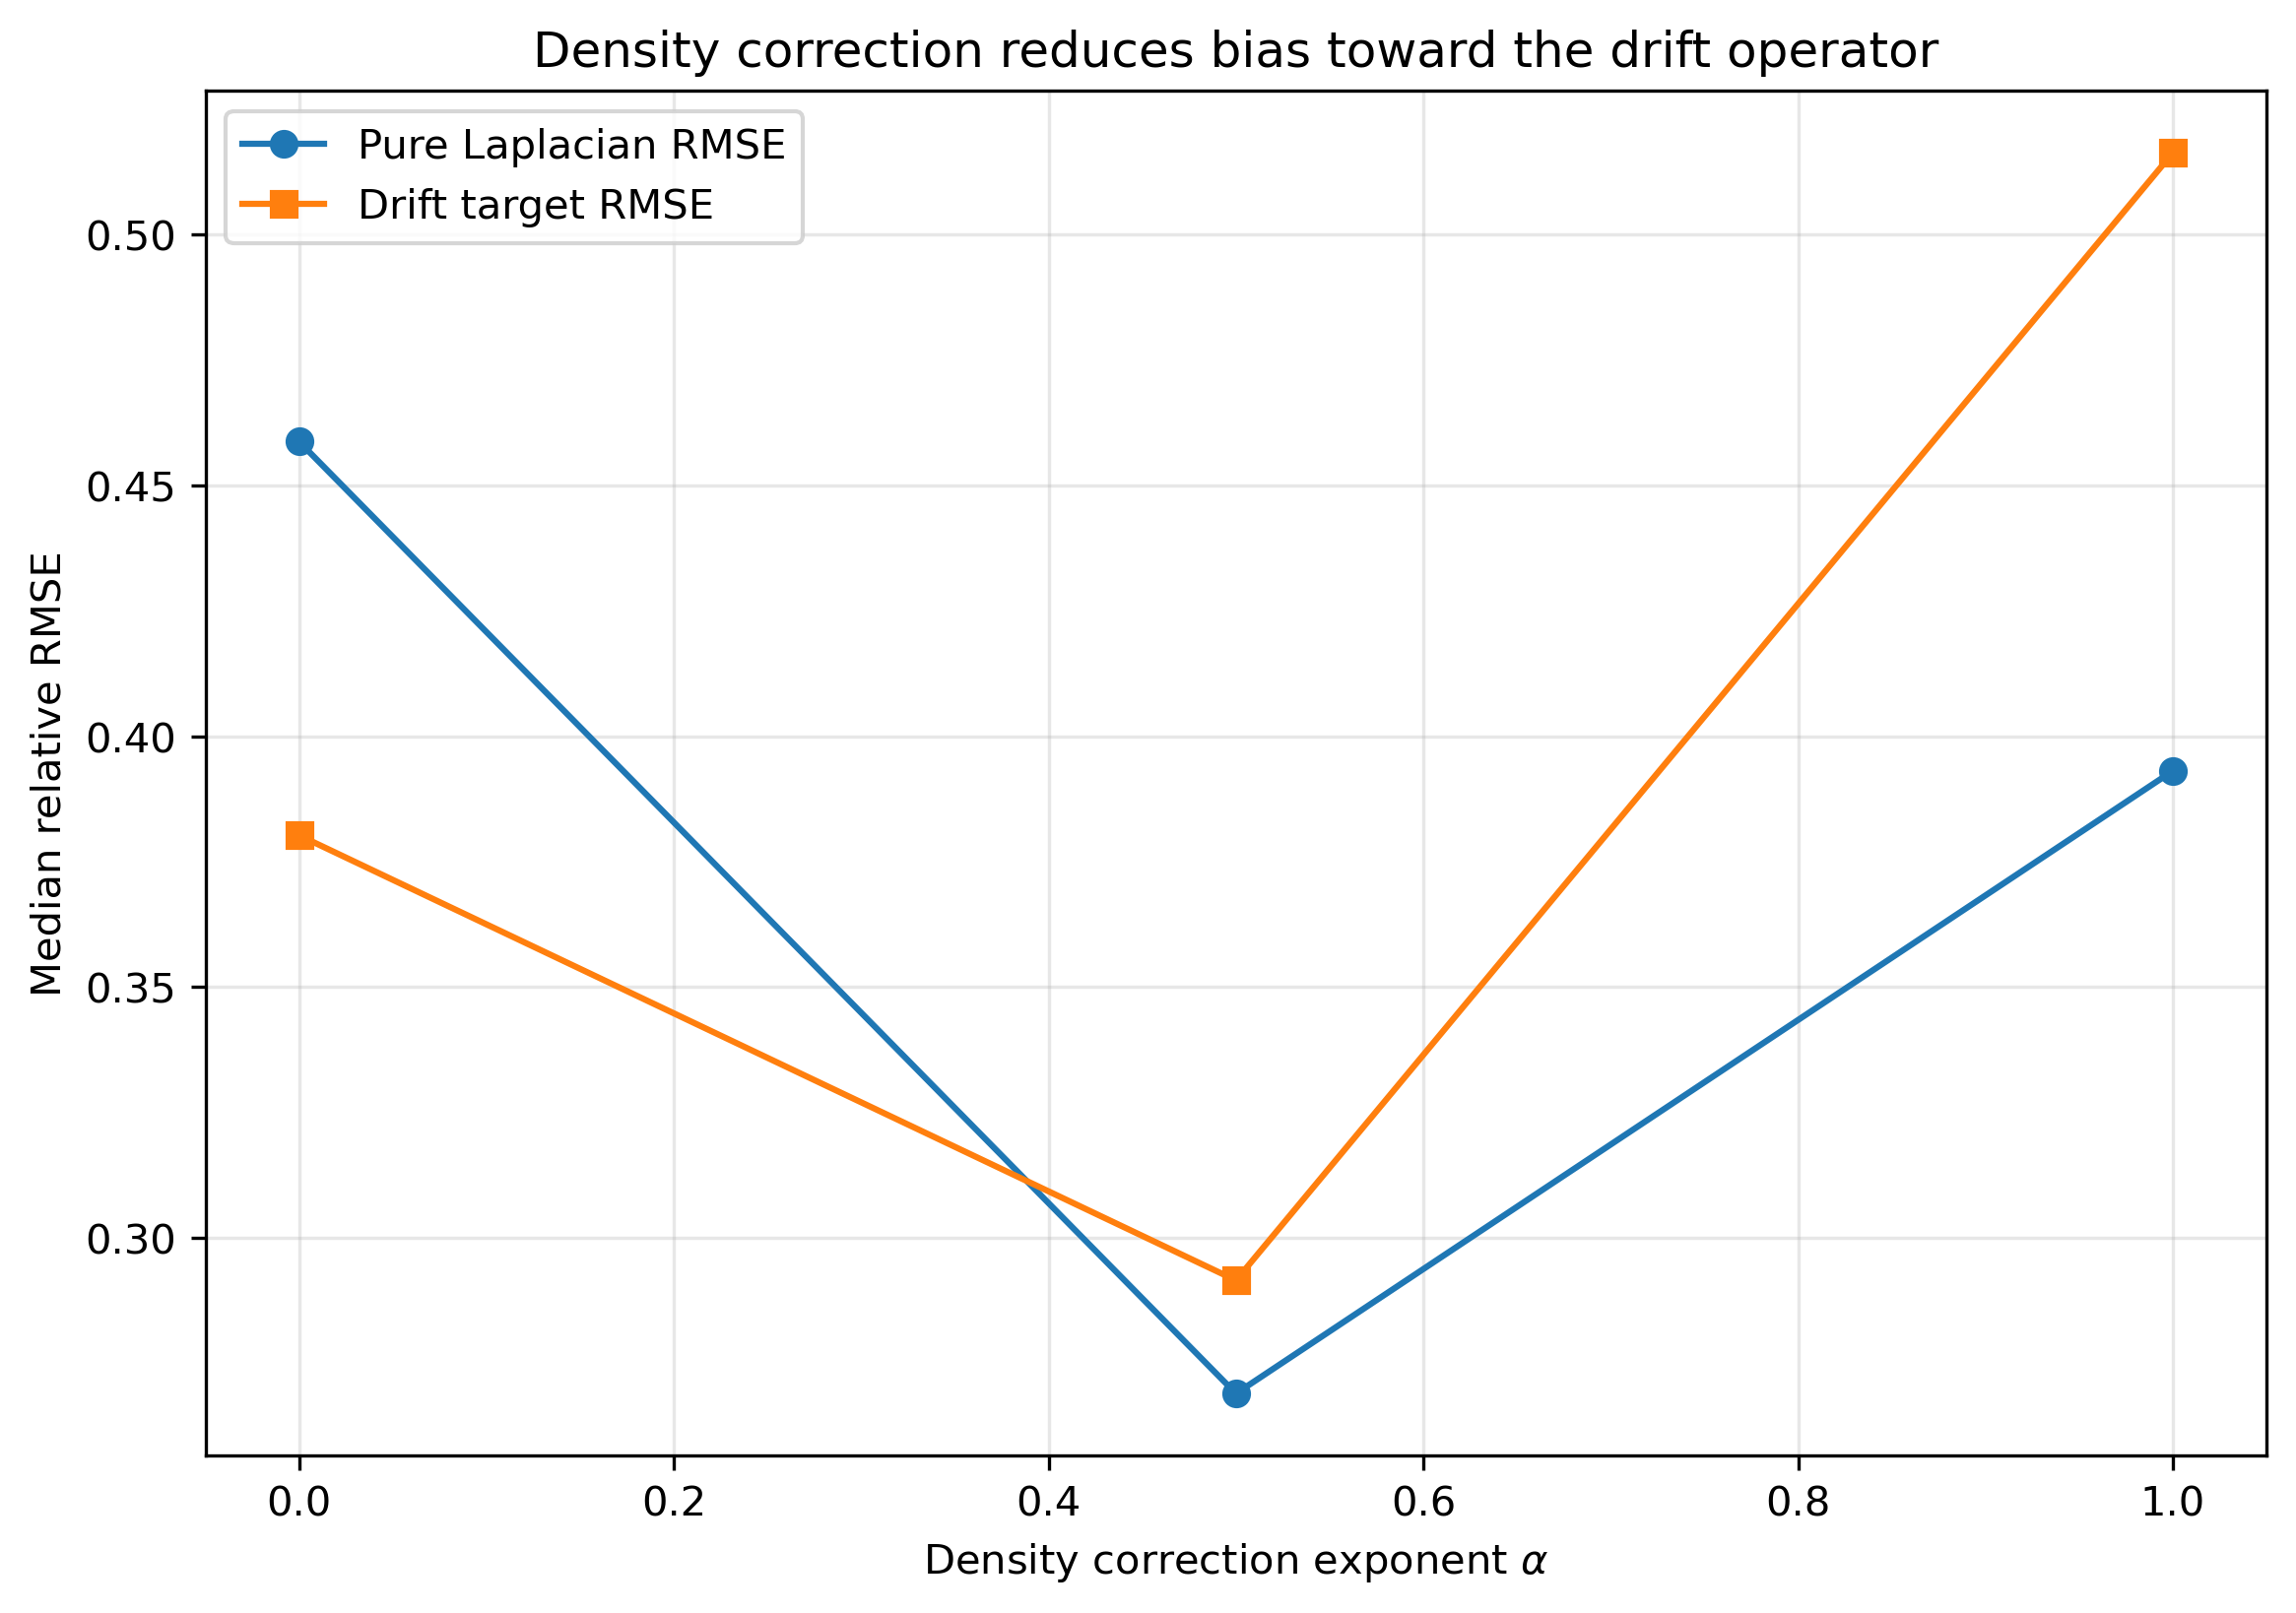
\includegraphics[width=0.88\textwidth]{figures/fig11_density_corrected_rmse_summary.png}
\caption{
Density correction for the symmetric combinatorial operator. In this finite-\(N\)
test, \(\alpha=1/2\) reduces the density bias and nearly flattens the graph
degree distribution.
}
\label{fig:density-corrected}
\end{figure}

\subsection{Diffusion-maps Markov generator}

To test the standard diffusion-maps convention, define
\begin{equation}
K_{ij}^{(\alpha)}
=
\frac{W_{ij}}
{q_i^\alpha q_j^\alpha}.
\end{equation}

The row-normalized Markov matrix is
\begin{equation}
P_{ij}^{(\alpha)}
=
\frac{K_{ij}^{(\alpha)}}
{\sum_j K_{ij}^{(\alpha)}}.
\end{equation}

The corresponding generator is
\begin{equation}
G^{(\alpha)}
=
\frac{I-P^{(\alpha)}}{\epsilon}.
\end{equation}

This is the convention in which \(\alpha=1\) is expected to remove sampling
density bias and recover the pure Laplace--Beltrami operator.

On the same non-uniform \(S^1\) test, the Markov-generator results are:

\begin{table}[htbp]
\centering
\begin{tabular}{rrr}
\toprule
\(\alpha\) & Median pure RMSE & Median drift RMSE \\
\midrule
0 & 0.3757 & 0.2521 \\
0.5 & 0.2343 & 0.2858 \\
1 & 0.1216 & 0.3680 \\
\bottomrule
\end{tabular}
\caption{
Diffusion-maps Markov-generator test on the same non-uniform \(S^1\) density.
In the Markov convention \(G^{(\alpha)}=(I-P^{(\alpha)})/\epsilon\), the
expected choice \(\alpha=1\) gives the best recovery of the pure Laplacian.
}
\label{tab:diffusion-maps-generator}
\end{table}

The best pure Laplacian recovery is
\begin{equation}
\alpha=1,\qquad
\epsilon=0.08,\qquad
\mathrm{RMSE}_{\rm pure}=0.0441.
\end{equation}

The same row has
\begin{equation}
\mathrm{RMSE}_{\rm drift}=0.3161.
\end{equation}

Thus the diffusion-maps Markov generator resolves the apparent anomaly:
\(\alpha=1/2\) is favoured only in the finite-\(N\) symmetric combinatorial
construction, whereas \(\alpha=1\) is favoured in the row-normalized
diffusion-maps convention.

\begin{figure}[htbp]
\centering
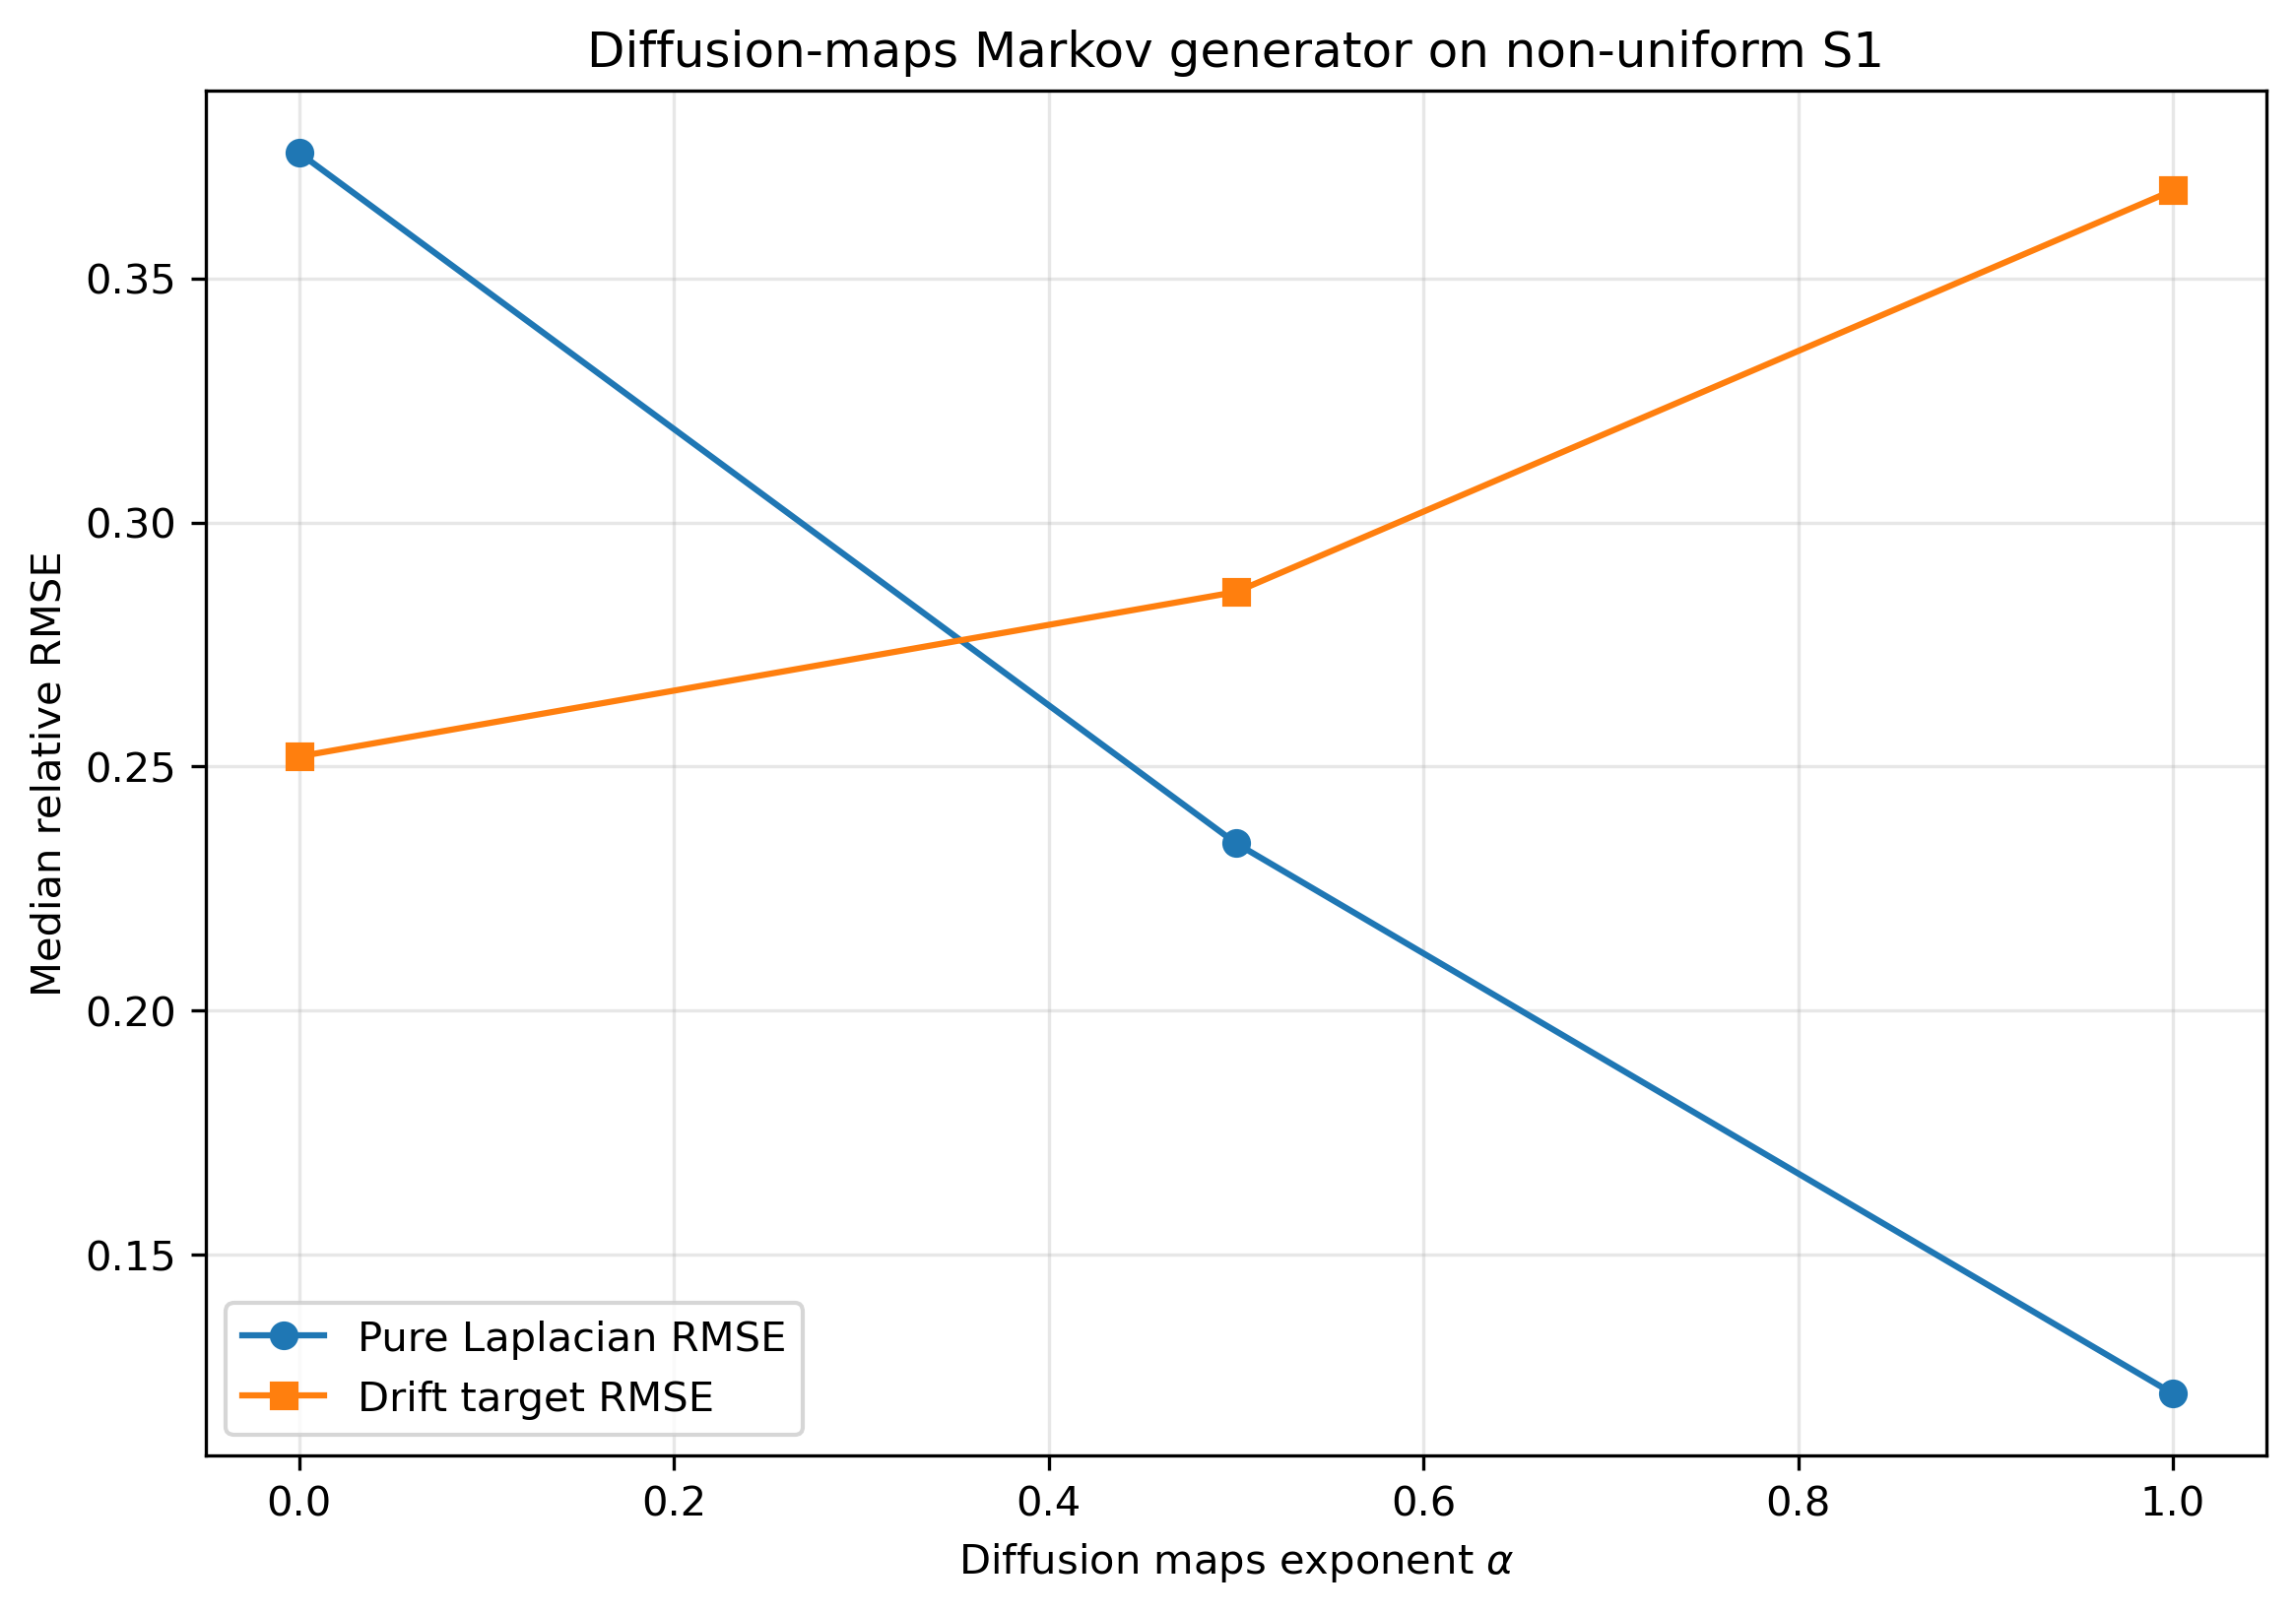
\includegraphics[width=0.86\textwidth]{figures/fig12_diffusion_maps_alpha_summary.png}
\caption{
Diffusion-maps Markov-generator comparison. In the row-normalized Markov
convention, \(\alpha=1\) gives the smallest median RMSE against the pure
Laplace--Beltrami target.
}
\label{fig:diffusion-maps-alpha}
\end{figure}

\section{Relation to mutual-information graphs}

The numerical and analytical tests in this paper use local Gaussian kernels.
BuP, however, starts from mutual information:
\begin{equation}
W_{ij}=I(i:j).
\end{equation}

Therefore, the bridge from this paper to full BuP requires a local-kernel
hypothesis:
\begin{equation}
I(i:j)\simeq F(d_g(x_i,x_j)),
\end{equation}
with a local regime in which \(F\) admits a diffusion-kernel approximation.

A schematic example is
\begin{equation}
I(i:j)
\sim
\exp\left[-\frac{d_g(x_i,x_j)^2}{4\epsilon_{\rm ent}}\right]
\end{equation}
at short entanglement distance.

This paper does not prove that arbitrary mutual-information graphs satisfy
this assumption. Instead, it establishes the normalization and density
correction required once the local-kernel regime is present.

\section{Implications for SPARC and SLACS graphs}

The density issue is not merely technical. Several BuP graphs used in the
phenomenological programme are not uniformly sampled. In particular:

\begin{itemize}
\item SPARC-inspired graphs may be baryon-weighted;
\item SLACS-inspired graphs may be lensing-weighted;
\item micro-closure graphs may contain nontrivial entanglement-density profiles.
\end{itemize}

Thus one should not apply the raw result
\begin{equation}
c_{N,\epsilon}L_{N,\epsilon}\to-\Delta_g
\end{equation}
blindly to those graphs.

The correct statement is:

\begin{quote}
For locally uniform entanglement density, the raw graph Laplacian converges to
the Laplace--Beltrami operator after the normalization
\[
c_{N,\epsilon}
=
\frac{1}
{\rho(4\pi)^{D/2}\epsilon^{D/2+1}}.
\]
For non-uniform entanglement density, the raw Laplacian contains density drift,
and a density-corrected graph Laplacian is required to recover a pure geometric
operator.
\end{quote}

This distinction strengthens rather than weakens the programme: it explains why
different BuP sectors require explicit normalization choices.

\section{Limitations}

The results of Paper 26 should be read with the following limitations.

\paragraph{Local Gaussian assumption.}
The analytical derivation assumes a local Gaussian kernel. Full mutual
information graphs require an additional physical argument establishing a local
diffusion-kernel regime.

\paragraph{Uniform density.}
The clean convergence to \(-\Delta_g\) holds under locally uniform density.
Non-uniform graphs require density correction or explicit drift terms.

\paragraph{Finite \(N\) effects.}
The numerical tests are finite. The sphere test is especially sensitive to
sampling and spectral multiplicities.

\paragraph{Operator convergence.}
The numerical evidence is primarily spectral and test-function based. A full
operator convergence theorem remains a mathematical target.

\paragraph{Normalization convention.}
Different graph Laplacians --- combinatorial, random-walk, symmetric normalized
and diffusion-maps Markov generators --- have different density-drift
structures. The normalization must be stated together with the operator
convention. In particular, the finite-\(N\) preference for \(\alpha=1/2\) in the
symmetric combinatorial construction should not be confused with the standard
diffusion-maps Markov result, where \(\alpha=1\) gives the best recovery of the
pure Laplace--Beltrami operator in our controlled test.

\section{Conclusion}

Paper 26 establishes the normalization of the local unnormalized graph
Laplacian required for convergence to the Laplace--Beltrami operator.

For a compact \(D\)-dimensional manifold with locally uniform density,
\begin{equation}
\rho=\frac{N}{\Vol(M)},
\end{equation}
the result is
\begin{equation}
\boxed{
L_{N,\epsilon}f
\simeq
-\rho(4\pi)^{D/2}\epsilon^{D/2+1}\Delta_g f.
}
\end{equation}

Therefore,
\begin{equation}
\boxed{
c_{N,\epsilon}
=
\frac{1}
{\rho(4\pi)^{D/2}\epsilon^{D/2+1}}
}
\end{equation}
gives
\begin{equation}
\boxed{
c_{N,\epsilon}L_{N,\epsilon}\to-\Delta_g.
}
\end{equation}

The formula is validated on \(S^1\), \(T^2\), and \(S^2\), giving the concrete
normalizations
\begin{equation}
S^1:\quad
\frac{\sqrt{\pi}}{N\epsilon^{3/2}},
\qquad
T^2:\quad
\frac{\pi}{N\epsilon^2},
\qquad
S^2:\quad
\frac{1}{N\epsilon^2}.
\end{equation}

The non-uniform \(S^1\) tests show that the raw combinatorial Laplacian
develops a density drift. In the symmetric combinatorial family
\(D^{(\alpha)}-W^{(\alpha)}\), the correction
\[
W_{ij}\mapsto\frac{W_{ij}}{\sqrt{q_iq_j}}
\]
substantially improves recovery of the pure Laplace--Beltrami operator in the
finite-\(N\) controlled setting. In the diffusion-maps Markov-generator
convention
\[
G^{(\alpha)}=\frac{I-P^{(\alpha)}}{\epsilon},
\]
the expected density-correcting choice \(\alpha=1\) gives the best recovery,
with a best pure-Laplacian RMSE of \(0.0441\).

Thus Paper 26 closes the principal normalization debt identified in Paper 25
and clarifies the density-correction required before applying the entanglement
Laplacian to non-uniform BuP graphs.

\begin{thebibliography}{9}

\bibitem{coifmanlafon}
R. R. Coifman and S. Lafon,
``Diffusion maps,''
\emph{Applied and Computational Harmonic Analysis} 21, 5--30 (2006).

\bibitem{belkinniyogi}
M. Belkin and P. Niyogi,
``Towards a theoretical foundation for Laplacian-based manifold methods,''
\emph{Journal of Computer and System Sciences} 74, 1289--1308 (2008).

\bibitem{singer}
A. Singer,
``From graph to manifold Laplacian: the convergence rate,''
\emph{Applied and Computational Harmonic Analysis} 21, 128--134 (2006).

\bibitem{paper25}
F. Hamdad,
``Paper 25 --- Variational Foundation of Bottom-Up Quantum Gravity,''
Bottom-Up Quantum Gravity Programme (2026).

\end{thebibliography}

\end{document}
